\documentclass[aps,preprintnumbers,showpacs,nofootinbib,superscriptaddress,floatfix]{revtex4}

\pdfoutput=1 % if your are submitting a pdflatex (i.e. if you have
             % images in pdf, png or jpg format)

%%%%%%%%%%%%%%%%%%%%%%%%%%%%
\usepackage{graphicx}
\usepackage{amssymb}
\usepackage{amsmath}
\usepackage{bm}
\usepackage{slashed}
\usepackage{datetime}
\usepackage{mciteplus}
\usepackage{multirow}
\usepackage{color}

%%%%%%%%%%%%%%%%%%%%%%%%%%%

\newcommand{\xbj}{x_B}
\newcommand{\zh}{z_h}

%% macro to draw particularly short right arrows. Choose one of the two
\newcommand{\smarrow}{\mbox{\raisebox{-4.5pt}[0pt][0pt]{$\hspace{-1pt} 
		\vec{\phantom{v}}$}}}
%\newcommand{\smarrow}{\mbox{\raisebox{0.5pt}{\tiny $\hspace{-1.5pt} \rightarrow 
%\hspace{-8.25pt}{\color{white} \rule[1pt]{1.5pt}{0.5pt}} \hspace{4pt} $}} }

%% names of experiments + MINUIT
\newcommand{\hermes}{\textsc{Hermes }}
\newcommand{\compass}{\textsc{Compass }}
\newcommand{\minuit}{\textsc{Minuit }}

%% macro to manage T versus perp notation
\newcommand{\T}{\perp}
\newcommand{\Tperp}{T}
\newcommand{\bT}{\zeta_T}
\newcommand{\bb}{\zeta}

%%%%%%%%%%%%%%%%%%%%%%%%%%%%%%%%%%%%%%%%%%%%%%%

\begin{document}
\allowdisplaybreaks[2]


\title{
Extraction of partonic transverse momentum distributions 
from semi-inclusive deep
inelastic scattering, Drell-Yan scattering, and Z-boson production.
}

\author{Alessandro Bacchetta}
\email{alessandro.bacchetta@unipv.it}
\affiliation{Dipartimento di Fisica, Universit\`a di Pavia, via Bassi 6,
  I-27100 Pavia} 
\affiliation{INFN Sezione di Pavia, via Bassi 6, I-27100 Pavia, Italy}

\author{Filippo Delcarro}
\email{filippo.delcarro01@ateneopv.it}
\affiliation{Dipartimento di Fisica, Universit\`a di Pavia, via Bassi 6,
  I-27100 Pavia} 
\affiliation{INFN Sezione di Pavia, via Bassi 6, I-27100 Pavia, Italy}

\author{Cristian Pisano}
\email{alessandro.bacchetta@unipv.it}
\affiliation{Dipartimento di Fisica, Universit\`a di Pavia, via Bassi 6,
  I-27100 Pavia} 
\affiliation{INFN Sezione di Pavia, via Bassi 6, I-27100 Pavia, Italy}

\author{Marco Radici}
\email{marco.radici@pv.infn.it}
\affiliation{INFN Sezione di Pavia, via Bassi 6, I-27100 Pavia, Italy}

\author{Andrea Signori}
\email{asignori@jlab.org}
\affiliation{Theory Center, Thomas Jefferson National Accelerator Facility, 12000 Jefferson Avenue, Newport News, VA 23606, USA}
%\affiliation{Department of Physics and Astronomy, VU University Amsterdam, De
% Boelelaan 1081, NL-1081 HV Amsterdam, the Netherlands}
%\affiliation{Nikhef, Science Park 105, NL-1098 XG Amsterdam, the
% Netherlands}

\begin{abstract}
We present an extraction of unpolarized partonic transverse momentum
distributions (TMDs) 
from a simultaneous fit of available data measured in semi-inclusive deep inelastic scattering 
and in Drell-Yan processes with the production of photon and $Z$ bosons. 
To connect data at different scales, we use TMD evolution at next-to-leading logarithmic accuracy. The
analysis is restricted to the low-transverse-momentum region, with no matching
to fixed-order calculations at high transverse momentum. We introduce specific
choices to deal with TMD evolution at low scales, of the order of 1 GeV$^2$.
This could be considered as a first attempt at a global fit of TMDs.
\end{abstract}

\preprint{JLAB THY 17-****}

\date{\today, \currenttime}

\pacs{13.60.Le, 13.87.Fh,14.20.Dh}

\maketitle
\tableofcontents

\newpage
%%%%%%%%%%%%%%%%%%%%%%%%%%%%%%%%%%%%%%%%%%%%%%%%%%%%%%%%%%%%%%%%%%
\section{Introduction}
\label{s:intro}
%%%%%%%%%%%%%%%%%%%%%%%%%%%%%%%%%%%%%%%%%%%%%%%%%%%%%%%%%%%%%%%%%%

Parton distribution functions describe the internal structure of the nucleon
in terms of its elementary constituents (quarks and gluons). They cannot be
easily computed from first principles, because they require the ability to
carry out Quantum Chromodynamics (QCD) calculations in a nonperturbative
regime. Many experimental observables in hard scattering experiments
involving hadrons are related to parton distribution functions (PDFs) and
fragmentation functions (FFs), in a way that is specified by factorization
theorems (see, e.g., Refs.~\cite{Collins:1989gx,Collins:2011zzd}). 
These theorems also elucidate the universality properties of PDFs and FFs
(i.e., the fact that they are the same in different processes) 
and their evolution equations (i.e., how they get modified by the change in
the hard scale of the process). 
Availability of measurements of different processes in different
experiments makes it possible to test the reliability of factorization
theorems and extract PDFs and FFs through so-called global fits. 
On the other side, the knowledge of PDFs and FFs allows us
to make predictions for other hard hadronic processes. 
These general statements apply equally well to
standard collinear PDFs and FFs and to transverse-momentum-dependent parton
distribution functions (TMD PDFs) and fragmentation functions (TMD FFs). 
Collinear PDFs
describe the distribution of partons integrated over all components of
partonic momentum except the one collinear to the parent hadron; hence,
collinear PDFs
are functions only of the parton longitudinal momentum fraction $x$. 
TMD PDFs (or TMDs for short) 
include also the dependence on transverse momentum components $k_{\T}^2$. 
They can be interpreted as three-dimensional generalizations of collinear PDFs.
Similar arguments apply to collinear FFs and TMD FFs~\cite{Angeles-Martinez:2015sea}.

There are several differences between collinear and TMD distributions. From
the formal point of view, factorization theorems for the two types of
functions are qualitatively different, implying also different universality
properties and evolution equations~\cite{Rogers:2015sqa}. From the
experimental point 
of view, observables related to TMDs require the measurement of some transverse
momentum component much smaller than the hard scale of the
process~\cite{Bacchetta:2016ccz,Radici:2016hbh}.  For
instance, Deep-Inelastic Scattering (DIS) is characterized by a hard scale represented by the
4-momentum squared of the virtual photon ($-Q^2$). In inclusive DIS this is
the only scale of the process, and access is limited to collinear PDFs
and FFs. In semi-inclusive DIS (SIDIS) also the transverse momentum of the
outgoing  
hadron ($P_{hT}$) can be measured~\cite{Mulders:1995dh,Bacchetta:2006tn}. 
If $P_{hT}^2\ll Q^2$, TMD
factorization can be applied and the process is sensitive to
TMDs~\cite{Collins:2011zzd}. 

%If $P_{h\perp}^2\sim Q^2$ or if the measurement is integrated over $P_{h\perp}$,
%collinear factorization applies and the process is sensitive to collinear
%PDFs. 

If polarization is taken into account, several TMDs can be
introduced~\cite{Mulders:1995dh,Boer:1997nt,%quark twist 2, spin 1/2
Bacchetta:2000jk,%quark twist 2, spin 1
Mulders:2000sh,%gluon twist 2, spin 1/2
Boer:2016xqr%gluon twist 2, spin 1
}. Attempts to extract some of them have already been presented in the past~\cite{Bacchetta:2011gx,Anselmino:2012aa,Echevarria:2014xaa,Anselmino:2016uie,%Sivers
Lu:2009ip,Barone:2015ksa,%Boer-Mulders
Lefky:2014eia,%pretzelosity
Anselmino:2013vqa,Kang:2015msa%Collins
}.  In
this work, we focus on the simplest ones, i.e., the unpolarized TMD
PDF $f_1^q(x,k_{\T}^2)$ and the unpolarized TMD
FF $D_1^{q \to h}(z,P_{hT}^2)$, where $z$ is
  the fractional energy carried by the detected hadron $h$. Despite their
  simplicity, the phenomenology of these unpolarized TMDs present several
  challenges~\cite{Signori:2016lvd}: the functional form of TMDs at low
  partonic transverse momentum, its possible dependence on the parton
  flavor~\cite{Signori:2013mda}, the implementation of TMD
  evolution~\cite{Bacchetta:2015ora,Rogers:2015sqa}, the matching to
  fixed-order calculations in collinear
  factorization~\cite{Collins:2016hqq}. 

We take into consideration three kinds of processes: semi-inclusive DIS, and
Drell--Yan processes (DY) with the production of virtual photons and $Z$
bosons. To date, they represent 
all possible processes
  where experimental information is available for unpolarized TMD
  extractions. 
The only important
process currently missing is electron-positron annihilation, which is
particularly important for the determination of TMD
FFs~\cite{Bacchetta:2015ora}. This work can therefore be considered as the
first attempt at a global fit of TMDs.  

The paper is organized as follows. In Sec.~\ref{s:theory}, the general
formalism for TMDs in SIDIS and DY processes is briefly outlined, including a
description of the assumptions and approximations in the phenomenological
implementation of TMD evolution equations. In Sec.~\ref{s:data_analysis}, the criteria
for selecting the data analyzed in the fit are summarized and commented. In
Sec.~\ref{s:results}, the results of our global fit are presented and
discussed. In Sec.~\ref{s:conclusions}, we summarize the results and present an outlook for future analyses. 
   

%%%%%%%%%%%%%%%%%%%%%%%%%%%%%%%%%%%%%%%%%%%%%%%%%%%%%%%%%%%%%%%%%%
\section{Formalism}
\label{s:theory}
%%%%%%%%%%%%%%%%%%%%%%%%%%%%%%%%%%%%%%%%%%%%%%%%%%%%%%%%%%%%%%%%%%

\textcolor{red}{AS: Shall we add pictures for the kinematics of SIDIS and DY data ? E.g. see Fig. 1 in~\cite{Signori:2013mda}.}

%%%%%%%%%%%%%%%%%%%%%%%%%%%%%%%%%%%%
\subsection{Semi-inclusive DIS}
\label{ss:SIDIS_formalism}

In one-particle SIDIS, a lepton $\ell$ with momentum $l$ scatters 
off a hadron target $N$ with mass $M$ and momentum
$P$. In the final state, the scattered lepton momentum 
$l'$ is measured together with
one hadron $h$ with mass $M_h$
and momentum $P_h$. The corresponding reaction formula is  
\begin{equation}
  \label{e:sidis}
\ell(l) + N(P) \to \ell(l') + h(P_h) + X \, .
\end{equation}
The space-like momentum transfer is $q = l - l'$, with $Q^2 = - q^2$. We
introduce the usual invariants  
\begin{align}
  \label{e:xyz}
x &= \frac{Q^2}{2\,P\cdot q},
&
y &= \frac{P \cdot q}{P \cdot l},
&
z &= \frac{P \cdot P_h}{P\cdot q},
&
\gamma &= \frac{2 M x}{Q} .
\end{align}

The available data refer to SIDIS hadron multiplicities, namely to the differential number of hadrons produced per corresponding inclusive DIS event. In terms of cross sections, we define the multiplicities as
\begin{equation}
m_N^h (x,z,|\bm{P}_{h\Tperp}|, Q^2) = \frac{d \sigma_N^h / ( dx  dz d|\bm{P}_{h\Tperp}| dQ^2) }
                                                                   {d\sigma_{\text{DIS}} / ( dx dQ^2 ) }\, ,
\label{e:multiplicity}
\end{equation}
where $d\sigma_N^h$ is the differential cross section for the SIDIS process and $d\sigma_{\text{DIS}}$ is the corresponding inclusive one, 
and where \( \bm{P}_{h\Tperp} \) is the component of \( \bm{P}_{h} \) transverse to \( \bm{q} \). 
In the single-photon-exchange approximation, the multiplicities can be written as ratios of
structure functions (see \cite{Bacchetta:2006tn} for details):
\begin{equation}
m_N^h (x,z,|\bm{P}_{h\Tperp}|, Q^2) =   
\frac{2 \pi\,|\bm{P}_{h\Tperp}| F_{UU ,T}(x,z,\bm{P}_{h\Tperp}^2, Q^2) + 2 \pi
  \varepsilon |\bm{P}_{h\Tperp}| F_{UU ,L}(x,z,\bm{P}_{h\Tperp}^2, Q^2)}
        {F_{T}(x,Q^2) + \varepsilon  F_{L}(x,Q^2)} \, ,
 \label{e:mFF}
\end{equation} 
where
\begin{align}
\varepsilon &= \frac{1-y -\frac{1}{4} \gamma^2 y^2}{1-y+\frac{1}{2} y^2 +\frac{1}{4} \gamma^2 y^2} \ .
\end{align}  
%\textcolor{red}{and the structure function $F_{XY,Z}$ corresponds to a lepton with polarization $X$ scattering on a target with polarization $Y$ by exchanging a virtual photon in a polarization state $Z$.}

The semi-inclusive cross section can be expressed in a factorized form in
terms of TMDs only in the kinematical limits $M^2 \ll Q^2$ and $\bm{P}_T^2 \ll
Q^2$. In these limits, the structure function $F_{UU,L}$ of Eq.~\eqref{e:mFF}
can be neglected~\cite{Bacchetta:2008xw}. 
 The structure function $F_L$ in the denominator contains contributions
 involving powers of the strong coupling constant $\alpha_S$ at an order that
 goes beyond the level reached in this analysis; 
hence, it will be
 consistently neglected (for measurements and
 estimates of the $F_L$ structure function see, e.g.,
 Refs.~\cite{Chekanov:2009na,Andreev:2013vha} and references therein).  

To express the structure functions in terms of TMD PDFs and FFs, 
we rely on the factorized formula 
for SIDIS~\cite{Collins:1981uk,Collins:1984kg,Ji:2002aa,Ji:2004wu,%
Collins:2011zzd,Aybat:2011zv,GarciaEchevarria:2011rb,Echevarria:2012pw,%
Collins:2012uy}:  
\begin{align}
\label{e:SIDISkT}
   F_{UU,T}(x,z, \bm{P}_{h \Tperp}^2, Q^2) &= \sum_a \mathcal{H}_{UU,T}^{a}(Q^2;\mu^2) \\ 
      &\times x \int d\bm{k}_\T^{} \, d\bm{P}_\T^{} \,  f_1^a\big(x,\bm{k}_{\T}^2; \mu^2 \big) \, D_{1}^{a\smarrow h}\big(z,\bm{P}_{\T}^2; \mu^2 \big) \,
      \delta \big(z {\bm k}_{\T} - {\bm P}_{h \Tperp} + {\bm P}_{\T}\big)
\nonumber\\&
\nonumber + Y_{UU,T}\big(Q^2, \bm{P}_{h\Tperp}^2\big) + \mathcal{O}\big(M^2/Q^2\big) \, .
\end{align} 
Here, $\mathcal{H}_{UU,T}$ is the hard scattering part; $f_1^a(x,\bm{k}_{\T}^2;
\mu^2)$ is the TMD distribution of unpolarized partons with flavor $a$ in an unpolarized
proton, carrying longitudinal momentum fraction $x$ and transverse momentum
$\bm{k}_\T$ at the factorization scale $\mu^2$, which in the following we
choose to be equal to $Q^2$.  The $D_1^{a\smarrow h}(z, \bm{P}_{\T}^2;
\mu^2)$ is the TMD fragmentation function describing the fragmentation of an unpolarized parton with flavor $a$ into
an unpolarized hadron $h$ carrying longitudinal momentum fraction $z$ and
transverse momentum 
$\bm{P}_\T$. The term $Y_{UU,T}$ is introduced to ensure a matching
to the perturbative fixed-order calculations at higher transverse momenta. 

In our analysis, we neglect any correction of the order of $M^2/Q^2$ or higher
to  Eq.~\eqref{e:SIDISkT}.
At large $Q^2$ this is well justified. 
However, fixed-target DIS experiments typically 
collect a large amount of data
at relatively low $Q^2$ values, where the reliability of these assumptions
should be tested in future studies. The reliability
of the theoretical description of SIDIS at low $Q^2$ has been recently
discussed in Refs.~\cite{Boglione:2016bph,Moffat:2017sha}.
 
Eq.~\eqref{e:SIDISkT} can be expanded in powers
of $\alpha_S$. In the present analysis, we 
will consider only the leading order terms in $\alpha_S$, i.e., stop at
order $\alpha_S^0$. In this case 
$\mathcal{H}^a_{UU,T} (Q^2, \mu^2) \approx e_a^2$
and $Y_{UU,T}\approx 0$. 
However, perturbative corrections include large logarithms $L \equiv
\log\big(z^2 Q^2/P_{hT}^2\big)$, so that $\alpha_S L \approx 1$.
In the present analysis, we will take into account all 
powers of the form $\alpha_S^n L^{2n-1} \approx 1$ (Leading Logarithms --LL) 
and 
$\alpha_S^n L^{n-1} \approx 1$ (Next-to-Leading Logarithms -- NNL).

In these approximations (LO in $\alpha_S$ and NLL), only the first term in
Eq.~\eqref{e:SIDISkT} is relevant (often in the
literature this has been called $W$ term). We expect this term to provide a
good description of the
structure function only in the region where $P_{hT}^2/z^2 \ll Q^2$. 
It can happen that $Y_{UU,T}$, defined
in the standard way (see, e.g., Ref.~\cite{Collins:1984kg}), gives large
contributions also in this region, but it is admissible to
redefine it in order to avoid this problem~\cite{Collins:2016hqq}. 
We leave a detailed treatment of the matching to the high $P_{hT}^2 \approx Q^2$
region to future investigations.   

To the purpose of applying TMD evolution equations, 
 need to calculate the Fourier transform of the the part of 
Eq.~\eqref{e:SIDISkT} involving TMDs. The structure function thus reduces to 
\begin{align}
\label{e:SIDISkTFF}
   F_{UU,T}(x,z, \bm{P}_{h \Tperp}^2, Q^2) &\approx 2\pi \sum_a e_a^2 x 
       \int_0^{\infty} {d \bT} \bT J_0\big(\bT |\bm{P}_{hT}|/z\big)
      \tilde{f}_1^a\big(x, \bT^2:Q^2\big) \tilde{D}_1^{a\smarrow h}\big(z, \bT^2;
      Q^2 \big) 
\nonumber \, .
\end{align} 
\textcolor{red}{ E' questa la formula usata nel codice, o serve dire altro?}
where we introduced the Fourier transforms of the TMD PDF and FF according to
\begin{align} 
\tilde{f}_1^a\big(x, \bT^2;\mu^2\big) &=
% \frac{1}{2\pi}\int_0^{\infty} d^2 \bm{k}_\T  e^{i \bm{k}_\T \cdot \bm{b}_T}
%       f_1^a\big(x, \bm{k}_\T^2;\mu^2\big)
%\\ &= 
\int_0^{\infty} d |\bm{k}_\T| 
                |\bm{k}_\T|J_0\big(\bT |\bm{k}_\T|\big) 
       f_1^a\big(x, \bm{k}_\T^2;\mu^2\big),
\\
\tilde{D}_1^{a\smarrow h}\big(z, \bT^2; \mu^2 \big) &=
% \frac{1}{2\pi} \int_0^{\infty} \frac{d^2 \bm{P}_\T}{z^2} e^{i (\bm{P}_\T \cdot \bm{b}_T)/z}
%       D_1^{a\smarrow h}\big(z, \bm{P}_{\T}^2; \mu^2 \big)
%\\ &=
\int_0^{\infty} \frac{d |\bm{P}_{\T}|}{z^2} |\bm{P}_{\T}| 
                                             J_0\big(\bT |\bm{P}_{\T}|/z\big)
       D_1^{a\smarrow h}\big(z, \bm{P}_{\T}^2; \mu^2 \big).
\end{align}  


%%%%%%%%%%%%%%%%%%%%%%%%%%%%%%%%%%%%
\subsection{Drell--Yan processes}
\label{ss:DY_formalism}

In a Drell--Yan process, two hadrons $A$ and $B$ with momenta $P_A$ and $P_B$
collide at a center-of-mass energy squared $s = (P_A + P_B)^2$ 
and produce a virtual photon or a $Z$ boson plus hadrons. 
The boson decays into a
lepton-antilepton pair. The reaction formula is
\begin{equation}
A(P_A)+B(P_B)\to [\gamma^*/Z + X \to] \ell^+(l) + \ell^-(l') + X.
\end{equation} 
The invariant mass of the virtual photon is $Q^2=q^2$ with $q = l + l'$. 
We introduce the rapidity of the virtual photon/Z boson
\begin{equation}
\eta=\frac{1}{2}\log\bigg(\frac{q^0+q_z}{q^0-q_z}\bigg)\  .
\end{equation} 
where the $z$ direction is defined along the momentum of hadron A.

The cross section can be written in terms of structure
functions~\cite{Boer:2006eq,Arnold:2008kf}. For our purposes, we need the unpolarized 
cross section
integrated over $d\Omega$ and over the azimuthal angle of the virtual photon, 
\begin{align}
\label{e:dsigma_gZ}
\frac{d\sigma}{dQ^2\, dq_T^2\,d\eta} &= \sigma_0^{\gamma,Z}
\bigg(F_{UU}^1 + \frac{1}{2} F_{UU}^2\bigg). 
\end{align} 
The elementary cross sections are
\begin{align}
\sigma_0^{\gamma} &= \frac{4\pi^2 \alpha^2_{\rm em}}{3 Q^2 s},
&
\sigma_0^Z &= 
%\frac{\sqrt{2} \pi G_F M_Z^2}{s}
\frac{\pi^2 \alpha_{\rm em}}{s \sin^2{\theta_W} \cos^2{\theta_W}}
B_R(Z\rightarrow \ell^+\ell^-)
\delta(Q^2 - M_Z^2), 
\end{align} 
where $\theta_W$ is Weinberg's angle, $M_Z$ is the mass of the $Z$ boson, and
$B_R$ is the branching ratio for the $Z$ boson decay in two leptons.
We adopted the narrow-width approximation, i.e., we neglect contributions for 
$Q^2 \neq M_Z^2$. 
We used the values 
$\sin^2 \theta_W= 0.2313$, $M_Z = 91.18$ GeV, and 
$B_R(Z\rightarrow \ell^+\ell^-)=3.366$.  
Similarly to the SIDIS case, in the kinematical limit $q_T^2 \ll Q^2$ 
the structure function $F_{UU}^2$ can be neglected 
(for measurement and estimates of this
structure function see, e.g.,
Ref.~\cite{Lambertsen:2016wgj} and references therein). 
%Similar reasons as for the semi-inclusive DIS case leads us to neglecting
%the structure function $F_{UU}^2$.

The longitudinal momentum fractions can be written in terms of
rapidity in the following way 
\begin{align}
x_A &= \frac{Q}{\sqrt{s}} e^{\eta},
&
x_B &= \frac{Q}{\sqrt{s}} e^{-\eta}.
\label{xab}
\end{align} 
Some experiments use the variable $x_F$, which is connected to the other
variables  by the following relations
\begin{align}
\label{e:eta_xf}
\eta &= \sinh^{-1}\bigg(\frac{\sqrt{s}}{Q}\frac{x_F}{2}\bigg),
& 
x_{A} &= \sqrt{\frac{Q^2}{s} + \frac{x_F^2}{4}} + \frac{x_F}{2},
&
x_B &= x_A - x_F.  
\end{align} 

The structure function $F_{UU}^1$ can be written as
\begin{align}
\label{e:DYkT}
   F_{UU}^1(x_A,x_B, \bm{q}_{T}^2, Q^2) &= \sum_a \mathcal{H}_{UU}^{1 a}(Q^2;\mu^2) \\ 
      &\times x_A x_B \int d\bm{k}_{\T A}^{} \, d\bm{k}_{\T B}^{} 
\,  f_1^a\big(x_A,\bm{k}_{\T A}^2; \mu^2 \big) 
\, f_{1}^{\bar{a}}\big(x_B,\bm{k}_{\T B}^2; \mu^2 \big) \,
      \delta \big({\bm k}_{\T A} - {\bm q}_T + {\bm k}_{\T B}\big)
\nonumber\\&
\nonumber + Y_{UU}^1\big(Q^2, \bm{q}_T^2\big) + \mathcal{O}\big(M^2/Q^2\big) \, .
\end{align} 


As in the SIDIS case, in our analysis we neglect $Y_{UU}$ term
and we consider the hard coefficients only up to leading order in
the couplings, i.e.,
\begin{align} 
{\cal H}_{UU, \gamma}^{1 a}(Q^2;\mu^2) &\approx \frac{e_a^2}{N_c},
&
{\cal H}_{UU, Z}^{1 a}(Q^2;\mu^2) &\approx \frac{V_a^2+A_a^2}{N_c} \ ,
\end{align}  
where\footnote{We remind the reader that the value of weak isospin $I_3$ is equal to $+1$ for $u$, $c$, $t$ and
  $-1$ for $d$, $s$, $b$.}
\begin{align}
V_a & = I_{3a} - 2 e_{a} \sin \theta_W \  ,
&
A_a & = I_{3a} \  .
\end{align} 

The structure function can be conveniently expressed as a Fourier transform of
the right-hand side of Eq.~\eqref{e:DYkT} as 
\begin{align}
\label{e:DYkTFF}
   F_{UU}^1(x_A,x_B, \bm{q}_T^2, Q^2) &\approx
 2\pi \sum_a {\cal H}_{UU}^{1 a} \,x_a x_B \int_0^{\infty} d \bT \bT\, J_0\big( \bT |\bm{q}_T|\big)\ 
      \tilde{f}_1^a\big(x_A, \bT^2;\mu^2\big) \   \tilde{f}_1^{\bar{a}}\big(x_B, \bT^2;\mu^2 \big)  \, .
\end{align} 

\textcolor{red}{ Stessa osservazione che in SIDIS: \`e questa la formula usata nel codice, o serve dire altro?}



%%%%%%%%%%%%%%%%%%%%%%%%%%%%%%%%%%%%
\subsection{TMDs and their evolution}
\label{ss:TMDevo}

Following the formalism of Refs.~\cite{Collins:2011zzd,Aybat:2011zv}, the
unpolarized TMD distribution and fragmentation functions in configuration
space for a parton flavor $a$ at a certain scale $\mu^2$ can be written as 
\begin{align}   
\widetilde{f}_1^a (x,  \bT^2; Q^2) &= \sum_{i=q,\bar q,g} \bigl( C_{a/i} \otimes f_1^i \bigr) (x; \mu_b^2) 
\  e^{S (\mu_b^2, Q^2)} \  e^{g_K(\bT) \ln (Q^2 / Q_0^2)} \  \widetilde{f}_{1 {\rm NP}}^a (x, \bT^2) \ ,
\label{e:TMDevol1} \\
\widetilde{D}_1^{a\to h} (z, \bT^2; \mu^2) &= \sum_{i=q,\bar q,g} \bigl( \hat{C}_{a/i} \otimes D_1^{i\to h} \bigr) (z; \mu_b^2) \  e^{S (\mu_b^2, Q^2)} \  e^{g_K( \bT) \ln (Q^2 / Q_0^2)} \  \widetilde{D}_{1 {\rm NP}}^{a\to h} (z, \bT^2) \  .
\label{e:TMDevol2}
\end{align}

The $C$ and $\hat{C}$ are perturbatively calculable Wilson coefficients for
the TMD distribution and fragmentation functions, respectively. They are
convoluted with the corresponding collinear functions according to 
\begin{align}
\bigl( C_{a/i} \otimes f_1^i \bigr) (x; \mu_b^2) &=
  \int_x^1 \frac{du}{u}\  
        C_{a/i} \Big( \frac{x}{u}, \alpha_S\big(\mu_b^2\big)  \Big) \  
        f_1^i (u; \mu_b^2) \  , 
\label{e:WC1} \\
\bigl( \hat{C}_{a/i} \otimes D_1^{i\to h} \bigr) (z; \mu_b^2) &= \int_z^1 \frac{du}{u}\  \hat{C}_{a/i} \left( \frac{z}{u}, \alpha_S\big(\mu_b^2\big) \right) \  D_1^{i\to h} (u; \mu_b^2) \  . 
\label{e:WC2}
\end{align}
In the present analysis, we consider only the leading-order term
in the $\alpha_S$ expansion, i.e., 
\begin{align} 
C_{a/i} \Big( \frac{x}{u}, \alpha_S\big(\mu_b^2\big)  \Big) &\approx
\delta_{ai} \delta(1-x/u),
&
\hat{C}_{a/i} \Big( \frac{z}{u}, \alpha_S\big(\mu_b^2\big)  \Big) &\approx
\delta_{ai} \delta(1-z/u).
\end{align}  
As a consequence, the expression for the evolved TMD functions reduces to
\begin{align}   
\widetilde{f}_1^a (x,  \bT^2; Q^2) &= f_1^a (x ; \mu_b^2) 
\  e^{S (\mu_b^2, Q^2)} \  e^{g_K(\bT) \ln (Q^2 / Q_0^2)} \  \widetilde{f}_{1 {\rm NP}}^a (x, \bT^2) \ ,
\label{e:TMDevol1b} \\
\widetilde{D}_1^{a\to h} (z, \bT^2; Q^2) &= D_1^{a\to h} (z; \mu_b^2) \  e^{S (\mu_b^2, Q^2)} \  e^{g_K( \bT) \ln (Q^2 / Q_0^2)} \  \widetilde{D}_{1 {\rm NP}}^{a\to h} (z, \bT^2) \  .
\label{e:TMDevol2b}
\end{align}

The Sudakov exponent $S$ 
%in Eqs.~\eqref{e:TMDevol1b} and \eqref{e:TMDevol2b} 
can be written as
\begin{equation} 
S(\mu_b^2,Q^2)=-\int_{\mu_b^2}^{Q^2}{d\mu^2\over \mu^2}
\bigg[A\Big(\alpha_s(k_T)\Big)\ln\bigg({Q^2\over \mu^2}\bigg) 
+ B\Big(\alpha_s(k_T)\Big) \bigg] \;.
\label{e:Sudakov} 
\end{equation} 
Functions $A$ and $B$ have perturbative expansions of the form
\begin{align}
A\left(\alpha_s(k_T)\right) &= \sum_{k=1}^{\infty}A_k
\bigg(\frac{\alpha_S}{\pi} \bigg),
&
B\left(\alpha_s(k_T)\right) &= \sum_{k=1}^{\infty}B_k
\bigg(\frac{\alpha_S}{\pi} \bigg).
\end{align} 
To NNL accuracy, we need the following 
terms \cite{Davies:1984hs,Collins:1984kg}
\begin{align}
A_1&= C_F, 
&
A_2&=
\frac{1}{2} C_F  \bigg[
C_A \bigg( \frac{67}{18} - \frac{\pi^2}{6} \bigg)
- \frac{5}{9} N_f \bigg],
&
B_1&= - \frac{3}{2}C_F.
\end{align} 
We use the approximate analytic expression for $\alpha_S$ at NLO with the
$\Lambda_{\text{QCD}}=$ 340 MeV, 296 MeV, 214 MeV for three, four, five
flavors, respectively, corresponding to a value of $\alpha_S(M_Z)=0.117$. 
We fix the flavor thresholds at $m_c=1.5$ GeV and 
$m_b= 4.7$ GeV. The integration of the Sudakov exponent in
Eq.~\eqref{e:Sudakov} can
be done analytically (for the complete expressions see, e.g.,
Refs.~\cite{Frixione:1998dw,Bozzi:2005wk,Echevarria:2012pw}).  


%\textcolor{red}{The convolutions are only valid for small $\bT \ll
%  1/\Lambda_{\rm QCD}$. At larger $\bT$, the TMDs need to match the
%  nonperturbative expressions $\widetilde{f}_{1 \rm NP}^a$ and
%  $\widetilde{D}_{1 {\rm NP}}^{a\to h}$, respectively, that must be
%  constrained by fitting experimental data. The evolution of TMDs from the
%  initial scale $Q_0$ to $\mu$ is carried out through perturbatively
%  calculable Sudakov factors $S$ and $\hat{S}$, respectively, and through a
%  nonperturbative universal term $g_K$ at large $\bT$ that accounts for the
%  radiation of soft gluons emitted by the considered parton. } 

The collinear PDFs in Eqs.~\eqref{e:TMDevol1b}, \eqref{e:TMDevol2b} are computed at a
scale $\mu_b^2$, which is also the lower limit of integration in the Sudakov
exponent in Eq.~\eqref{e:Sudakov}. We choose it to be
\begin{align} 
\mu_b &= \frac{2 e^{-\gamma_E}}{\bar{\bb}_{\ast}} \  ,
\label{e:mub}
\end{align}  
where $\gamma_E$ is the Euler constant and
\begin{align} 
\bar{\bb}_{\ast} &\equiv \bb_{\rm max} \Bigg(\frac{1-e^{- \bT^4 / \bb_{\rm max}^4} }{1-e^{- \bT^4 / \bb_{\rm min}^4}} \Bigg)^{1/4} .
\label{e:b*}
\end{align}  
This variable replaces the simple dependence upon $\bT$ in the
  convolutions of Eqs.~\eqref{e:WC1}, \eqref{e:WC2} and in the perturbative
  Sudakov factors $S$ and $\hat{S}$; namely, in the perturbative parts of the
  TMD definitions of Eqs.~\eqref{e:TMDevol1},~\eqref{e:TMDevol2}. In fact, at
  large $\bT$ these parts are no longer reliable. Therefore, the
  $\bar{\bb}_{\ast}$ is chosen to saturate on the maximum value $\bb_{\rm max}$,
  as suggested by the CSS 
  formalism~\cite{Collins:2011zzd,Aybat:2011zv}.\footnote{We remind that
  different schemes are possible to deal with 
the high-$\bT$ region like the so-called ``complex-$\bb$
prescription''~\cite{Laenen:2000de}.}
On the other hand, at
small $\bT$ the TMD formalism is not reliable and should be 
matched to the fixed-order collinear
calculations. The way
the matching is implemented is arbitrary.  In any case, the TMD contribution
can be arbitrarily modified at small $\bT$. In our approach, we choose to
saturate 
$\bar{\bb}_{\ast}$  at
the minimum value $\bb_{\rm min}\propto 1/Q$. With the appropriate choices, 
for $\bT=0$ the Sudakov exponent vanishes, as it
should~\cite{Parisi:1979se,Altarelli:1984pt}. 
Our choice partially corresponds to modifying the resummed logarithms as in
Ref.~\cite{Bozzi:2010xn} and to other similar modifications proposed in the
literature~\cite{Boer:2014tka,Collins:2016hqq}. One advantage of these kind of
prescriptions is that by integrating over the impact parameter $\bT$, the
collinear expression for the cross section, in terms of collinear PDFs, is
recovered, at least at leading order~\cite{Collins:2016hqq}.

The values of $\bb_{\rm max}$ and
$\bb_{\rm min}$ could
be regarded as arbitrary scales separating perturbative from nonperturbative
regimes. 
We choose to fix them to the
values 
\begin{align}
\bb_{\rm max} &= 2 e^{-\gamma_E}  \text{  GeV}^{-1} = 1.123 \text{  GeV}^{-1}, 
&
\bb_{\rm min} &= 2 e^{-\gamma_E}/Q \ .
\label{e:bminmax}
\end{align} 
The motivations are the following: 
\begin{itemize}
\item{} with the above choices, the scale $\mu_b$ is
  constrained between 1 GeV and $Q$, so that the collinear PDFs are never
  computed at a scale lower than 1 GeV and the lower limit of the integrals
  contained in the definition of the perturbative Sudakov factor can never
  become larger than the upper limit;
\item{} at $Q_0 = 1$ GeV, $\bb_{\rm max} = \bb_{\rm min}$ and there are no evolution effects; the TMD is
simply given by the corresponding collinear function multiplied by a
nonperturbative contribution depending on $k_\T$ (plus possible corrections of
order $\alpha_S$ from the Wilson coefficients) .
\end{itemize} 

Following Refs.~\cite{Nadolsky:1999kb,Landry:2002ix,Konychev:2005iy}, for the
nonperturbative Sudakov factor we make the traditional choice $g_K (\bT) = -
g_2 \bT^2 / 2$ with $g_2$ a free parameter. Recently, several alternative
forms have been proposed~\cite{Aidala:2014hva,Collins:2014jpa} including the
suggestion of not including such term~\cite{D'Alesio:2014vja}. 

In this analysis, for the collindear PDFs $f_1^a$ we adopt the GJR08FFnloE
set~\cite{Gluck:2007ck} through the LHAPDF library~\cite{Buckley:2014ana}, and
for the collinear fragmentation functions 
the DSS14 NLO set for
pions~\cite{deFlorian:2014xna} and the DSS07 NLO set for
kaons~\cite{deFlorian:2007aj}.\footnote{After the completion of our analysis, 
a new set of kaon
  fragmentation function was presented in Ref.~\cite{deFlorian:2017lwf}.} We
will comment on the use of other PDF sets in Sec.~\ref{ss:replica105}.

We parametrize the intrinsic nonperturbative parts of the TMDs in the
following ways
\begin{align}
\widetilde{f}_{1 {\rm NP}}^a (x, \bT^2) &= \frac{1}{2\pi}
        e^{-\langle \bm{k}_{\T a}^2 \rangle \frac{\bT^2}{4}}
        \bigg( 1 - \frac{\lambda \langle \bm{k}_{\T a}^2 \rangle^2}{1+\lambda\langle \bm{k}_{\T a}^2 \rangle}  \frac{\bT^2}{4} \bigg)\  ,
\label{e:f1NP} \\
\widetilde{D}_{1 {\rm NP}}^{a \to h} (z, \bT^2) &= 
    \frac{ \langle \bm{P}_{\T a\to h}^2 \rangle \   e^{-\langle \bm{P}_{\T
          a\to h}^2 \rangle \frac{\bT^2}{4 z^2}}
        + \big(\lambda_F/z^2\big)    \langle \bm{P}_{\T a\to h}'^2 \rangle^2
    \left(1 - \langle \bm{P}_{\T a\to h}'^2 \rangle \frac{\bT^2}{4 z^2} \right)
         \  e^{- \langle \bm{P}_{\T a\to h}'^2 \rangle \frac{\bT^2}{4z^2}}}
     {2 \pi z^2 \Big(\langle \bm{P}_{\T a\to h}^2 \rangle + \big(\lambda_F/z^2\big)   \langle \bm{P}_{\T a\to h}'^2 \rangle^2\Big)} \  .
\label{e:D1NP}
\end{align} 
After performing the anti-Fourier transform, the $f_{1 \rm NP}$ and $D_{1\rm
  NP}$ in momentum space correspond to the normalized linear combination of
a Gaussian and a weighted Gaussian:
\begin{align} 
f_{1 {\rm NP}}^a (x, \bm{k}_{\T}^2) &= \frac{1}{\pi} \  
                        \frac{\big( 1 +\lambda \bm{k}_{\T}^2\big)}
                                {\langle \bm{k}_{\T a}^2 \rangle +\lambda \  \langle \bm{k}_{\T a}^2 \rangle^2}
                        \  e^{- \frac{\bm{k}_{\T}^2}{\langle \bm{k}_{\T a}^2 \rangle}} \  ,
\label{e:f1NPk}   \\
D_{1 {\rm NP}}^{a\to h} (z, \bm{P}_{\T}^2) &=  \frac{1}{\pi} \   
                  \frac{1}{\langle \bm{P}_{\T a\to h}^2 \rangle +
                    \big(\lambda_F/z^2\big) \langle \bm{P}_{\T a\to h}'^2 \rangle^2}
           \   \bigg( e^{- \frac{\bm{P}_{\T}^2}{\langle \bm{P}_{\T a\to h}^2 \rangle}}
                            + \big(\lambda_F/z^2\big)   \bm{P}_{\T}^2 \  
           e^{- \frac{\bm{P}_{\T}^2}{\langle \bm{P}_{\T a\to h}'^2 \rangle}} \bigg) \  .
\label{e:D1NPk}
\end{align} 
In the TMD PDF case, the Gaussian and the
weighted Gaussian have the same width, while in the fragmentation function, we
considered the possibility that the two Gaussian widths are different. 
We consider that the
Gaussian width of the TMD distribution depends 
on the parton flavor $a$ and on its fractional momentum $x$ according to
\begin{align} 
\big\langle \bm{k}_{\T a}^2 \big\rangle (x) &= \big\langle \hat{\bm{k}}_{\T a}^2 \big\rangle \;  
\frac{(1-x)^{\alpha} \  x^{\sigma} }{ (1 - \hat{x})^{\alpha} \  \hat{x}^{\sigma} } \, ,
\label{e:kT2_kin}
\end{align}
where $\alpha, \, \sigma,$ and $\big\langle \hat{\bm{k}}_{\T a}^2 \big\rangle \equiv \big\langle \bm{k}_{\T a}^2 \big\rangle (\hat{x})$ with $\hat{x} = 0.1$, are free parameters. Similarly, we have
\begin{align}  
\big\langle \bm{P}_{\T a \to h}^2 \big\rangle (z) &= \big\langle \hat{\bm{P}}_{\T a \to h}^2 \big\rangle \  
               \frac{ (z^{\beta} + \delta)\ (1-z)^{\gamma} }{ (\hat{z}^{\beta} + \delta)\   (1 - \hat{z})^{\gamma} } \, ,
 \label{e:PT2_kin}
 \end{align}
where $\beta, \, \gamma, \, \delta, $ and $\big\langle \hat{\bm{P}}_{\T a \to
  h}^2 \big\rangle \equiv \big \langle \bm{P}_{\T a \to h}^2 \big\rangle
(\hat{z})$ with $\hat{z} = 0.5$, are free parameters. The same functional form
applies also to the width of the weighted Gaussian. For simplicity, we
considered parameters $\beta$, $\delta$, and $\gamma$ to be the same for both
Gaussians, and keep a distinction only between parameters 
$\big\langle \hat{\bm{P}}_{\T a \to  h}^2 \big\rangle$ and
$\big\langle \hat{\bm{P}}_{\T a \to  h}^{\prime 2} \big\rangle$.
 
\textcolor{red}{Mention that also the other variance in the TMD FF has the same kinematic dependence.}
%For sake of simplicity, the $\beta, \, \gamma, \, \delta$ parameters are taken equal for all fragmentation channels~\cite{Signori:2013mda,Bacchetta:2015ora}. 
%




\newpage
%%%%%%%%%%%%%%%%%%%%%%%%%%%%%%%%%%%%%%%%%%%%%%%%%%%%%%%%%%%%%%%%%%
\section{Data analysis}
\label{s:data_analysis}
%%%%%%%%%%%%%%%%%%%%%%%%%%%%%%%%%%%%%%%%%%%%%%%%%%%%%%%%%%%%%%%%%%


The main goals of our work are to study the evolution of TMD parton distributions and fragmentation functions over a large enough range of energy and to test their universality among different processes. To achieve this we included measurements taken from SIDIS, Drell-Yan and $Z$ boson production from different experimental collaborations at different energy scales. \\
In this chapter we describe the data sets considered for each process and the reasons behind the kinematic cuts applied.

Tab.~\ref{t:data_SIDIS_proton} refers to the data sets for SIDIS off proton target (\hermes experiment) and presents their kinematic ranges. 
The same holds for Tab.~\ref{t:data_SIDIS_deuteron}, Tab.~\ref{t:data_DY}, Tab.~\ref{t:data_Z} for SIDIS off deuteron (\hermes and \compass experiments), Drell-Yan events at low energy and $Z$ boson production respectively. 
For each kinematic variable in all the considered data sets, we fit the average value in each bin.
 
%%%%%%%%%%%%%%%%%%%%%%%%%%%%%%%%%%%%
\subsection{Hermes data}
\label{ss:hermes}

The semi-inclusive DIS data are taken from \hermes~\cite{Airapetian:2012ki} and \compass~\cite{Adolph:2013stb} experiments. 
Both \hermes and \compass data have been already analyzed in previous works, e.g.~\cite{Signori:2013mda,Anselmino:2013lza}.

\hermes hadron multiplicities are measured in a fixed target experiment, colliding a $27.6\,GeV$ lepton beam on a hydrogen ($p$) or deuterium ($D$) gas target, for a total of 2688 points.\\
These are grouped in bins of $(x,z,Q^2,P_{hT})$ with the average values of $(x,Q^2)$ ranging from about $(0.04, 1.25\text{ GeV}^2)$ to $(0.4, 9.2\text{ GeV}^2)$. 
The collinear energy fraction $z$ in~\eqref{e:xyz} ranges in $0.1\leq z\leq 0.9$. The transverse momentum of the detected hadron satisfies $0.1 \text{ GeV} \leq \vert P_{hT} \vert \leq 1.3 \text{ GeV}$.
The peculiarity of \hermes SIDIS experiment lies in the ability of his detector to distinguish between pions and kaons in the final state, in addition to determine their momenta and charges.
The particle identification process distinguish the final data sets in eight different channels, one for every combination of target ($p,\,D$) and detected charged hadron ($\pi^\pm, \,  K^\pm$ ).
\hermes Collaboration published two distinct sets, characterized by the inclusion or subtraction of the vector meson contribution. In our work we considered only the data set where these contributions have been subtracted. \\


%%%%%%%%%%%%%%%%%%%%%%%%%%%%%%%%%%%%
\subsection{Compass data}
\label{ss:compass}

Compass collaboration extracted multiplicities of charge-separated but unidentified hadrons produced in SIDIS off a deuteron ($^6\text{LiD}$) target~\cite{Adolph:2013stb}.  The number of data is an order of magnitude higher compared to the \hermes experiment. \\
The data set are organised in multidimensional bins of $(x,z,Q^2,P_{h\Tperp})$, they cover a range in $(x,Q^2)$ from about $(0.005, 1.11\text{ GeV}^2)$ to $(0.09, 7.57\text{ GeV}^2)$ and the interval $0.2 \leq z \leq 0.8$. Similarly to \hermes, for \compass $P_{h\Tperp}^2 \lesssim 1$ GeV$^2$. 

The multiplicities published by \compass are affected by a normalization error (see the {\em erratum} to~\cite{Adolph:2013stb}), in order to avoid this issue we divide the data grouped in one of the bin characterized by a value of ($x, z, Q^2$) by the data point with the lowest $P_{hT}^2$ in that group.
We define the {\em normalized} multiplicity that result from this procedure as:
\begin{equation}
m_{\text{norm}}(x,z,\bm{P}_{h\Tperp}^2, Q^2) = \frac{m_N^h(x,z,\bm{P}_{h\Tperp}^2, Q^2)}{m_N^h (x,z,{\rm \min}[\bm{P}_{h\Tperp}^2], Q^2)} \ ,
\label{e:mult_norm}
\end{equation}
where the multiplicity $m_N^h$ is defined in~\eqref{e:multiplicity}. Fitting normalized multiplicities the first data point of each bin is considered as a fixed parameter and excluded from the degrees of freedom of the system.

The application of the TMD formalism to SIDIS crucially depends on the capability of identifying the current fragmentation region. This task has been recently discussed in~\cite{Boglione:2016bph}, where the authors point out a possible overlap among different  fragmentation regions when the hard scale $Q$ is sufficiently low. 
In this paper we do not tackle this problem and we leave it to future studies. As described in Tabs.~\ref{t:data_SIDIS_proton} and~\ref{t:data_SIDIS_deuteron}, we identify the current fragmentation region operating a cut on $z$ only, namely $0.2 < z < 0.74$.\footnote{The implementation of the ``collinearity'' criterion proposed in~\cite{Boglione:2016bph} crucially depends on the value of $\langle k_T^2 \rangle$, features that requires independent determinations of the partonic properties.}

%PhT <Min[0.2Q,0.7Qz]+0.5GeV
Another requirement for the applicability of TMD factorization is the presence of two separate hard scales in the process. In SIDIS, those are the $Q^2$ and $P_{hT}^2$, which should satisfy the hierarchy $\Lambda_{\text{QCD}}^2 \ll P_{hT}^2 \ll Q^2$. 
In order to satisfy $\Lambda_{\text{QCD}}^2 \ll Q^2$, we request $Q^2 > 1.4$ GeV$^2$. 
The second condition is $P_{hT}^2 \ll Q^2$, together with the further constraint  $P_{hT}^2/z^2 \ll Q^2$. In our analysis we relax
%~\footnote{\textcolor{red}{AS [comment to ourselves]: adding $0.5$ GeV might be a bit ``extreme'', since we could probe the $P_{hT} > Q$ region where a matching to fixed-order calculations should be taken into account.}} 
these conditions and implement them as $P_{hT} < \min[0.2\ Q, 0.7\ Qz] + 0.5$ GeV. The specific values of the terms are chosen to maximize the goodness of the fit procedure and not to exclude too many data points.
All these choices are summarized in Tabs.~\ref{t:data_SIDIS_proton} and~\ref{t:data_SIDIS_deuteron}.

%%%%%%%%%%%%%%%%%%%%%%%%%%%%%%%%%%%%
\subsection{Low-energy Drell-Yan data}
\label{ss:dy}

We analyze Drell-Yan events collected by fixed-target experiments at low-energy. These data set have been considered also in previous works, e.g.~\cite{DAlesio:2014mrz}. 
We used data sets from the E288 experiment~\cite{Ito:1980ev}, that measured the invariant dimuon cross section $E d^3\sigma / dp^3$ for the production of $\mu^+ \mu^-$ pairs from the collision of a proton beam with a fixed target, either composed of $Cu$ or $Pt$.
The measurements were repeated using proton incident energies of $200$, $300$ and $400$ $GeV$, producing three different data sets.
Their respective center of mass energies are $\sqrt{s}=19.4,23.8,27.4 Gev$.\\
We also included the set of measurements $E d^3\sigma / dp^3$ from E605~\cite{Moreno:1990sf}, extracted from the collision of a proton beam with an energy of $800$ $GeV$ ($\sqrt{s}=38.8 \text{ GeV}$) on a copper fixed target .\\

The explored $Q$ values are higher compared to the SIDIS case, as can be seen in Tab.~\ref{t:data_DY}. E288 provides data at fixed rapidity ,\textcolor{red}{ whereas E605 explores a range of values for $x_F$ (see~\eqref{e:eta_xf})}.  
As discussed for SIDIS data, we can apply TMD factorization if $\Lambda_{\text{QCD}}^2 \ll q_T^2 \ll Q^2$, where $q_T$ is the transverse momentum of the intermediate electroweak boson, reconstructed from the kinematics of the final state leptons. As done for SIDIS, we choose $q_T < 0.2\ Q + 0.5$ GeV. Again, the values of the coefficients are chosen to maximize the goodness of the fit and to not exclude too many points.
We consider the target nuclei as an ensemble composed by $40\%$ proton and $60\%$ nucleon, as suggested in~\cite{Ito:1980ev}, independent one from the other.

As we already observed, results from E288 and E605 experiments are reported as $\frac{Ed^3\sigma}{d^3p}$; this variable is related the differential cross section $d\sigma/dq_T$ in the following way~\cite{Olive:2016xmw} :

\begin{equation}
\frac{Ed^3\sigma}{d^3p}=\frac{d^3\sigma}{d\phi dy p_T dp_T} \Rightarrow \frac{d^2\sigma}{\pi dy d(p^2_T)}
\end{equation}

where the third term is the average over $\phi$.
The invariant dimuon cross section can be obtained from Eq.~\ref{e:dsigma_gZ} performing an integration of its terms over $Q^2$ and adding a factor $1/\pi$ to the result:

\begin{equation}
\frac{Ed^3\sigma}{d^3p} = \frac{1}{\pi} \int dQ^2 \frac{d\sigma}{dQ^2dq^2_T dy} .
\end{equation}

We checked that integrating in $Q^2$ only the prefactor $\sigma_q^\gamma$, defined in Eq.~\ref{e:elem_cs_sig0}, and not the entire term in Eq.~\ref{e:dsigma_gZ} (including then the convolution) introduces only a negligible error in the fit procedure:  

\begin{equation}
\frac{1}{\pi} \cdot \int dQ^2 \frac{4\pi \alpha^2_{em}}{3N_cQ^2 s} e_q^2 
= \frac{4\alpha_{em}^2}{3 N_c s} e_q^2 \ln \left( \frac{Q_f^2}{Q_i^2} \right) .
\end{equation}

%%%%%%%%%%%%%%%%%%%%%%%%%%%%%%%%%%%%
\subsection{Z-boson production data}
\label{ss:zboson}

In order to reach higher $Q$ and $q_T$ values, we also consider $Z$ boson production in collider experiments at Tevatron. 
We analyze data from CDF and D0, collected during Tevatron Run I~\cite{Affolder:1999jh,Abbott:1999wk} at $\sqrt{s}=1.8\text{ TeV}$ and Run II~\cite{Aaltonen:2012fi,Abazov:2007ac} at $\sqrt{s}=1.96\text{ TeV}$. CDF and D0 collaborations studied the differential cross section for $p\bar{p}\rightarrow Z/\gamma^* \rightarrow, e^+e^- + X$, that is the production of an $e^+e^-$ pairs from $p\bar{p}$ collision,  through an intermediate $Z$ vector boson. 

The invariant mass distribution peaks at the $Z$-pole, $Q=M_Z$, while the transverse momentum of the exchanged $Z$ ranges in $0< q_T < 20 \text{ GeV}$.
We use the same kinematic condition applied to Drell-Yan events:  $q_T < 0.2\ Q + 0.5$ GeV $ = 18.7$ GeV, since $Q$ is fixed to $M_Z$. 

The observable measured in CDF and D0 is $d\sigma /dq_T$,  apart from the case of D0 Run II, for which the published data refer to $1/\sigma \times d\sigma/dq_T$. In order to work with the same observable in all the cases considered, we multiply the D0-Run II data by the total cross section of the process $\sigma_{exp} = 255.8 \pm 16 \text{ pb}$~\cite{Abulencia:2005ix}. In this case, we add in quadrature the uncertainties of the total cross section and of the published data. 

We normalize our functional form with factors listed in Tab.~\ref{t:data_Z}. These are the same normalization factors used in~\cite{DAlesio:2014mrz} to fit $Z$ boson production and differ from the experimental ones. 

%\textcolor{red}{Cuts and reasons}\\


\renewcommand{\tabcolsep}{0.4pc} % enlarge column spacing
\renewcommand{\arraystretch}{1.3} % enlarge line spacing

%%%%%%%%%%%%%% Tab. SIDIS data off proton %%%%%%%%%%%%%%%%%%%%%%%%%%
\begin{table}[h!]
\begin{center}
\begin{tabular}{|c|c|c|c|c|}
 \hline
  & HERMES & HERMES & HERMES & HERMES \\
 ~          &  $p \to \pi^+$    &   $p \to \pi^-$    &  $p \to K^+$    &   $p \to K^-$               \\
 \hline
 Reference & \multicolumn{4}{c|}{\cite{Airapetian:2012ki}}        \\
\hline
\multirow{3}{*}{Cuts}             & \multicolumn{4}{c|}{$Q^2 > 1.4 \text{ GeV}^2$}     \\
             & \multicolumn{4}{c|}{$0.2 <z <0.74$}     \\
             & \multicolumn{4}{c|}{$P_{h \Tperp}< {\rm Min}[0.2\ Q, 0.7 \ Q z ] +0.5$ GeV}     \\
\hline
 Points         &  190 & 190 & 189 & 187       \\
 \hline
Max. $Q^2$      &  \multicolumn{4}{c|}{$9.2 \text{ GeV}^2 $}               \\
 \hline
$x$ range       & \multicolumn{4}{c|}{$0.06 < x < 0.4$ }                \\
\hline
%Notes         &\multicolumn{4}{c|}{ }   \\ 
%\hline 
%$\chi^2 /$points &4.24 & 3.49 & 0.63 & 1.00                \\
%\hline
\end{tabular}
\caption{Semi-inclusive DIS proton-target data (Hermes experiment).}
\label{t:data_SIDIS_proton}
\end{center}
\end{table}
%%%%%%%%%%%%%% Tab. SIDIS data off deuteron %%%%%%%%%%%%%%%%%%%%%%%%%%
\begin{table}[h!]
\begin{center}
\begin{tabular}{|c|c|c|c|c|c|c|}
 \hline
  & HERMES & HERMES & HERMES & HERMES & COMPASS & COMPASS\\
 ~          &  $D \to \pi^+$    &   $D \to \pi^-$    &  $D \to K^+$    &   $D \to K^-$      &  $D \to h^+$    &   $D \to h^-$            \\
 \hline
 Reference & \multicolumn{4}{c|}{\cite{Airapetian:2012ki}}        &\multicolumn{2}{c|}{\cite{Adolph:2013stb}} \\
\hline
\multirow{3}{*}{Cuts}             & \multicolumn{6}{c|}{$Q^2 > 1.4 \text{ GeV}^2$}     \\
             & \multicolumn{6}{c|}{$0.2 <z <0.7$}     \\
             & \multicolumn{6}{c|}{$P_{h \Tperp}< {\rm Min}[0.2\ Q, 0.7 \ Q z ] +0.5$ GeV}     \\
\hline
 Points         &  190 & 190 & 189 & 189   & 3125 & 3127   \\
 \hline
Max. $Q^2$      &  \multicolumn{4}{c|}{$9.2 \text{ GeV}^2 $}      & \multicolumn{2}{c|}{$10 \text{ GeV}^2 $}             \\
 \hline
$x$ range       & \multicolumn{4}{c|}{$0.06 < x < 0.4$ }    &  \multicolumn{2}{c|}{$0.006 < x < 0.12$ }             \\
\hline
Notes         &\multicolumn{4}{c|}{ }   & \multicolumn{2}{c|}{Observable: $\displaystyle m_{\text{norm}}(x,z,\bm{P}_{h\Tperp}^2, Q^2)$, eq.~\eqref{e:mult_norm}}  \\
%Notes         &\multicolumn{4}{c|}{ }   & \multicolumn{2}{c|}{Observable: $\displaystyle \frac{m_N^h
%    (x,z,\bm{P}_{h\Tperp}^2, Q^2)}{m_N^h (x,z,{\rm Min}[\bm{P}_{h\Tperp}^2], Q^2)}$}             \\
\hline 
%$\chi^2 /$points &3.06 & 2.53 & 1.04 & 3.18    &  1.48        &    0.96             \\
%\hline
\end{tabular}
\caption{Semi-inclusive DIS deuteron-target data (Hermes and Compass experiments).}
\label{t:data_SIDIS_deuteron}
\end{center}
\end{table}
%%%%%%%%%%%%%% Tab. Drell-Yan data low Q %%%%%%%%%%%%%%%%%%%%%%%%%%
\begin{table}[h!]
\begin{center}
%\newcommand{\m}{\hphantom{$-$}}
%\newcommand{\cc}[1]{\multicolumn{1}{c}{#1}}
\renewcommand{\tabcolsep}{0.4pc} % enlarge column spacing
\renewcommand{\arraystretch}{1.2} % enlarge line spacing
\begin{tabular}{|c|c|c|c|c|}
 \hline
 ~                        &  E288 200    &  E288 300        &  E288 400          &  E605                \\
 \hline
Reference               &  \cite{Ito:1980ev}  &   \cite{Ito:1980ev}  &  \cite{Ito:1980ev}  &   \cite{Moreno:1990sf}  \\
\hline
Cuts             & \multicolumn{4}{c|}{$q_T < 0.2\ Q +0.5$ GeV}
\\
 \hline
 Points                   &      45      &   45             &       78           &     35               \\
 \hline
 $\sqrt{s}$               &    19.4 GeV   &   23.8 GeV        &      27.4 GeV    &  38.8 GeV           \\
\hline
$Q$ range                 &  4-9 GeV      &  4-9 GeV         &  5-9, 11-14 GeV   &  7-9, 10.5-18 GeV   \\
 \hline
 Kin. var.           & $\eta$=0.4         &  $\eta$=0.21          &   $\eta$=0.03         &    $-0.1<x_F< 0.2$         \\
\hline
%$ \chi^2  /$points      &  0.52        &    0.98           &       0.68         &   0.68     \\
%\hline
\end{tabular}
\caption{Low energy Drell-Yan data collected by the E288 and E605 experiments at Tevatron, with different center-of-mass energies.}
\label{t:data_DY}
\end{center}
\end{table}
%%%%%%%%%%%%%% Tab. Z data Tevatron %%%%%%%%%%%%%%%%%%%%%%%%%%
\begin{table}[h!]
\begin{center}
%\vskip 18pt
%\newcommand{\m}{\hphantom{$-$}}
%\newcommand{\cc}[1]{\multicolumn{1}{c}{#1}}
\renewcommand{\tabcolsep}{0.4pc} % enlarge column spacing
\renewcommand{\arraystretch}{1.2} % enlarge line spacing
\begin{tabular}{|c|c|c|c|c|}
 \hline
 ~                        & CDF Run I    &  D0 Run I        & CDF Run II        & D0 Run II      \\
 \hline
 Reference        &\cite{Affolder:1999jh} &\cite{Abbott:1999wk}&\cite{Aaltonen:2012fi}&\cite{Abazov:2007ac} \\
\hline
Cuts             & \multicolumn{4}{c|}{$q_T< 0.2\ Q +0.5 \text{ GeV}=18.7$ GeV}                                  \\
\hline
 Points                   &      31      &   14             &       37          &        8       \\
 \hline
 $\sqrt{s}$               &      1.8 TeV &   1.8 TeV        &       1.96 TeV    &       1.96 TeV   \\
 \hline
Normalization        &  1.114       &    0.992          &       1.049        &       1.048    \\
\hline
%$\chi^2 /$points      &  0.52        &    0.98           &       0.68         &   0.68     \\
%\hline
\end{tabular}
\caption{$Z$ boson production data collected by the CDF and D0 experiments at Tevatron, with different center-of-mass energies.}
\label{t:data_Z}
\end{center}
\end{table}
%%%%%%%%%%%%%%%%%%%%%%%%%%%%%%%%%%%%%%%%%%%%%%%%%%%%%%%%%%%%%%%



%%%%%%%%%%%%%%%%%%%%%%%%%%%%%%%%%%%%
\subsection{The replica method}
\label{ss:replica_method}

\textcolor{red}{AS: I edited a bit the text, but some overlap remains in this section with the text in~\cite{Signori:2013mda}.}

In this section we describe the replica method and we give a definition of the $\chi^2$ function minimized by the fit procedure.
The fit and the error analysis were carried out using a similar Monte Carlo approach as in Ref.~\cite{Bacchetta:2012ty,Signori:2013mda,Radici:2015mwa} and taking
inspiration from the work of the Neural-Network PDF (NNPDF) collaboration (see, e.g.,~\cite{Forte:2002fg,Ball:2008by,Ball:2010de}). 
The approach consists in creating $\mathcal{M}$ replicas of the data points. In each replica (denoted by the index $r$), each data point $i$ is shifted by a Gaussian noise with the same variance as the measurement. 
Each replica, therefore, represents a possible outcome of an independent experimental measurement, which we denote by $m_{N, r}^{h}(x, z, \bm{P}_{h\Tperp}^2, Q^2)$. 
The number of replicas is chosen so that the mean and standard deviation of the set of replicas accurately reproduces the original data points. We see that 200 replicas are sufficient for the purpose.

A minimization procedure is applied to each replica separately, by minimizing the following error function:~\footnote{Note that the error for each replica is taken to be equal to the error on the original data points. This is consistent with the fact that the variance of the $\mathcal{M}$ replicas should reproduce the variance of the original data points.}  
\begin{equation}
E_r^2(\{p\})=\sum_{i} 
\frac{\Bigl(m_{N, r}^{h}(x_i, z_i, \bm{P}_{h\Tperp i}^2, Q_i^2) - m_{N,  \mbox{\tiny theo}}^{h}(x_i, z_i, \bm{P}_{h\Tperp i}^2; \{p\})\Bigr)^2}
        {\Bigl( \Delta m_{N, \mbox{\tiny stat}}^{h\ 2} + \Delta m_{N, \mbox{\tiny sys}}^{h\ 2} \Bigr)(x_i, z_i, \bm{P}_{h\Tperp i}^2, Q^2_i) +\Bigl(\Delta m_{N, \mbox{\tiny theo}}^{h}(x_i, z_i, \bm{P}_{h\Tperp i}^2) \Bigr)^2}\  . 
\label{e:MC_chi2}
\end{equation}
The sum runs over the $i$ experimental points, including all species of targets $N$ and final-state hadrons $h$. 
In each $z$ bin for each replica the values of the collinear fragmentation functions $D_1^{a \smarrow h}$ are independently modified with a Gaussian noise with standard deviation equal to the theoretical error $\Delta D_1^{a\smarrow h}$. 
In this work we rely on different parametrizations for $D_1^{a \smarrow h}$: for pions we use the DSEHS analysis~\cite{deFlorian:2014xna} at NLO in $\alpha_s$; for kaons we use the DSS parametrization~\cite{deFlorian:2007aj} at LO in $\alpha_s$. 
The uncertainties $\Delta D_1^{a\smarrow h}$ are estimated from the plots in~\cite{Epele:2012vg}; they represents the only source of uncertainty in $\Delta m_{N,  {\rm theo}}^{h}$. 
Statistical and systematic experimental uncertainties $\Delta m_{N, \mbox{\tiny stat}}^{h}$ and $\Delta m_{N, \mbox{\tiny sys}}^{h}$ are taken from the experimental collaborations. 
We do not take into account the covariance among different kinematic bins. 

\minuit minimizes the error function in~\eqref{e:MC_chi2} calculating its gradient with respect to the vector of parameters $\{p\}$. 
The final outcome is a set of $\mathcal{M}$ different vectors of best-fit parameters, $\{ p_{0r}\},\; r=1,\ldots \mathcal{M}$, with which we can calculate any observable, its mean, and its standard deviation. 
The distribution of these values needs not to be necessarily Gaussian. In fact, in this case the $1 \sigma$ confidence interval is different from the 68\% interval. 
The latter can simply be computed for each experimental point by rejecting the largest and the lowest 16\% of the $\mathcal{M}$ values.   

Although the minimization is performed on the function defined in~\eqref{e:MC_chi2}, the agreement of the $\mathcal{M}$ replicas with the original data is better expressed in terms of a $\chi^2$ function defined as in~\eqref{e:MC_chi2} but with the replacement $m_{N, r}^{h} \to m_{N}^{h}$, i.e.,  with respect to the original data set. If the model is able to give a good description of the data, the distribution of the $\mathcal{M}$ values of $\chi^2$/d.o.f. should be peaked around one. 
%In practice, the rigidity of our functional form leads to higher $\chi^2$ values. 














%\newpage
%%%%%%%%%%%%%%%%%%%%%%%%%%%%%%%%%%%%%%%%%%%%%%%%%%%%%%%%%%%%%%%%%%
\section{Results}
\label{s:results}
%%%%%%%%%%%%%%%%%%%%%%%%%%%%%%%%%%%%%%%%%%%%%%%%%%%%%%%%%%%%%%%%%%

\textcolor{red}{AS: Filippo, can you please check the final plots? I can't run the notebooks in Dropbox because of a problem with Mathematica.}

In the following we detail the results of a fit to the data sets described in Sec.~\ref{s:data_analysis} with a a flavor-independent configuration for the transverse momentum dependence of unpolarized TMDs.
In Tab.~\ref{t:fl_ind_chi2} we present the total $\chi^2$. The number of degrees of freedom (d.o.f.) is given by the number of data points analyzed reduced by the number of free parameters in the error function. 
The overall quality of the fit is good, with a global $\chi^2$/d.o.f. $= 1.55 \pm 0.05$. Uncertainties are computed as the $68\%$ confidence level (C.L.) from the replica methodology. 
%%%%%%%%%%%%%%%% Tab. chi2 total  %%%%%%%%%%%%%%%%%%%%%%%%%%
\begin{table}[h!]
\small
  \centering
  \begin{tabular}{|c|c|c|c|}
\hline
\hline
%  \multicolumn{4}{|c|}{Parameters for TMD PDFs} \\
%  \hline
%  \hline
Points& Parameters & $\chi^2$& $\chi^2/$d.o.f. \\
\hline
8059 & 11  & $12629 \pm 363$ & $1.55 \pm 0.05$ \\
\hline
\hline
\end{tabular}
%  \begin{tabular}{|c|c|c|c|c|c|c|c|c|c|c|}
%Points& Parameters & $\chi^2$& $\chi^2/$d.o.f.& 
%                  Points &$\chi^2$& Points &$\chi^2$& Points &$\chi^2$ 
% \\ 
%      &    &    &  & HERMES    & HERMES   & COMPASS & COMPASS & DY \& Z & DY \& Z  \\
%\hline
%8156 & 11  & $12629 \pm 363$ & $1.55 \pm 0.05$ & 1737&  &6126 & & 293 &    \\
%\hline
%\hline
%\end{tabular}
\caption{Total number of points analyzed, number of free parameters and $\chi^2$ values.}
\label{t:fl_ind_chi2}
\end{table}
%%%%%%%%%%%%%%%%%%%%%%%%%%%%%%%%%%%%%%%%%%%%%%%%%%%%%%%



%========================================================
\subsection{Agreement between data and theory}
\label{ss:data_vs_theory}

The partition of the global $\chi^2$ among SIDIS off proton, SIDIS off deuteron, Drell-Yan and $Z$ production events is given in Tab.~\ref{t:fl_ind_chi2_eP},~\ref{t:fl_ind_chi2_eD},~\ref{t:fl_ind_chi2_DY},~\ref{t:fl_ind_chi2_Z} respectively. 


\subsubsection*{Semi-inclusive DIS}
\label{sss:SIDIS_agreement}

%%% CHI2 VALUES %%%

For SIDIS at \hermes off a proton, events with a kaon in the final state have in general a lower $\chi^2$. This is due to the large uncertainties for the kaon FFs. 
The major contribution to the $\chi^2$ comes from events with a $\pi^+$ in the final state. 
In~\cite{Signori:2013mda,Signori:2013gra} a poor agreement between experiment and theory (which relies on the DSS parametrization~\cite{deFlorian:2007aj} for collinear FFs) at the level of the collinear multiplicities affected the quality of the fit, especially for $\pi^\pm$. Instead, in this work we use a newer parametrization of the collinear FFs (DSEHS~\cite{deFlorian:2014xna}), based on a fit which includes \hermes collinear pion multiplicities. This significantly improves the agreement at the collinear level with respect to~\cite{Signori:2013mda,Signori:2013gra}. 
The poor $\chi^2$ for $\pi^\pm$ production off a proton at \hermes is mainly due to a bad agreement in the TMD multiplciities at low $z$ values (see the first two blocks from the top in Fig.~\ref{f:H_pions}). 
For kaon production off the proton at \hermes the agreement at low $z$ is better than for the pions (see the first two blocks from the top in Fig.~\ref{f:H_kaons}), which, combined with larger uncertainties, results in lower $\chi^2$.
%%%%%%%%%%%%%% Tab. chi2 SIDIS off proton %%%%%%%%%%%%%%%%%%%%%%%%%%
\begin{table}[h!]
\begin{center}
\begin{tabular}{|c|c|c|c|c|}
 \hline
\hline
  & HERMES & HERMES & HERMES & HERMES \\   
 &  $p \to \pi^+$    &   $p \to \pi^-$    &  $p \to K^+$    &   $p \to K^-$
 \\
 \hline
 Points         &  190 & 190 & 189 & 187       \\
 \hline
%$\chi^2$ &4.24 & 3.49 & 0.63 & 1.00                \\
$\chi^2 /$points &4.83 & 2.47 & 0.91 & 0.82   \\            
\hline
\hline
\end{tabular}
\caption{Number of points analyzed and $\chi^2$ values for SIDIS off a proton target.}
\label{t:fl_ind_chi2_eP}
\end{center}
\end{table}
%%%%%%%%%%%%%%%%%%%%%%%%%%%%%%%%%%%%%%%%%%%%%%%%%%%%%%%


For SIDIS at \hermes off a deuteron, the situation is slightly different with respect to the proton case.
For pion production the $\chi^2$ is lower with respect to the scattering off a proton because the experimental uncertainties for $D \to \pi^\pm$ are slightly larger than for $p \to \pi^\pm$ (compare the first two blocks from the top with the last two ones in Fig.~\ref{f:H_pions}).
On the contrary, for kaon production the $\chi^2$ is higher with respect to the scattering off a proton because the experimental uncertainties for $D \to K^\pm$ are slightly smaller than for $p \to K^\pm$ (compare the first two blocks from the top with the last two ones in Fig.~\ref{f:H_kaons}).

Fixing the target and comparing pion and kaon production at \hermes, we see that the $\chi^2$ for kaons is in general lower than for pions. This is because the theoretical uncertainty for $D_1^{a \to K}$ is larger than the one for $D_1^{a \to \pi}$~\cite{Epele:2012vg,Signori:2013mda}, even if the experimental uncertainties are in general smaller for kaons.

SIDIS at \compass involves scattering off deuteron only, $D \to h^\pm$, and we identify $h \equiv \pi$. 
The quality of the agreement between theory and \compass data is better than in the case of pion production at \hermes. This depends on at least two factors. First: the fit is essentially driven by the \compass data, since the number of points in \compass is much higher than in \hermes. Moreover, the observable that we fit for the case of \compass is the normalized multiplicity, defined in~\eqref{e:mult_norm}. This automatically eliminates any possible tension between theory and data due to normalization effects.
%%%%%%%%%%%%%% Tab. chi2 SIDIS off deuteron %%%%%%%%%%%%%%%%%%%%%%%%%%
\begin{table}[h!]
\begin{center}
\begin{tabular}{|c|c|c|c|c|c|c|}
 \hline
\hline
  & HERMES & HERMES & HERMES & HERMES & COMPASS & COMPASS\\
 ~          &  $D \to \pi^+$    &   $D \to \pi^-$    &  $D \to K^+$    &   $D \to K^-$      &  $D \to h^+$    &   $D \to h^-$            \\
\hline
 Points         &  190 & 190 & 189 & 189   & 3125 & 3127   \\
 \hline
%$\chi^2$ &4.24 & 3.49 & 0.63 & 1.00                \\
$\chi^2 /$points &3.46 & 2.00 & 1.31 & 2.54  & 1.11 & 1.61 \\            
 \hline
 \hline
\end{tabular}
\caption{Number of points analyzed and $\chi^2$ values for SIDIS off a deuteron target.} 
\label{t:fl_ind_chi2_eD}
\end{center}
\end{table}
%%%%%%%%%%%%%%%%%%%%%%%%%%%%%%%%%%%%%%%%%%%%%%%%%%%%%%%


%%% FIGURES %%%

Fig.~\ref{f:H_pions} presents the agreement between the theoretical formula in~\eqref{e:multiplicity} and the \hermes multiplicities for production of pions off a proton and a deuteron. 
Different $\langle x \rangle$, $\langle z \rangle$ and $\langle Q^2 \rangle$ bins are displayed as a funciton of the transverse momentum of the dected hadron $P_{hT}$.
The grey bands are an envelope of the $200$ replica of best-fit curves. For every point in $P_{hT}$ we apply a $68\%$ C.L. selection criterion. 
Points marked with different symbols and colors correspond to different $\langle z \rangle$ values. There is a strong correlation between $\langle x \rangle$ and $\langle Q^2 \rangle$ that does not allow to explore $x$ and $Q^2$ dependence of the TMDs separetely. 
We notice that the agreement tends to improve as we move to higher $Q^2$ values, where the kinematic approximations of factorization are more reliable. 
Moreover, for fixed $P_{hT}$ and $Q^2$, the agreement is in general better at higher $z$ values, which also resembles the kinematic condition $P_{hT}/z \lesssim Q$ for TMD factorization.

Fig.~\ref{f:H_kaons} has same content and notation as in Fig.~\ref{f:H_pions} but for kaons in the final state. Here we notice that the agreement at low $z$ tends to be better than in the previous case of pion production. 

In Fig.~\ref{f:C_pim} we present \compass normalized multiplicities (see~\eqref{e:mult_norm}) for production of $\pi^-$ off a deuteron for different $\langle x \rangle$, $\langle z \rangle$, and $\langle Q^2 \rangle$ bins as a funciton of the transverse momentum of the dected hadron $P_{hT}$. The circle around the first $P_{hT}$ point in each panel indicates that the first value is fixed and not fitted. 
The correlation between $x$ and $Q^2$ is less strong than at \hermes and this allows to study different $\langle x \rangle$ bins at fixed $\langle Q^2 \rangle$.
For the highest $Q^2$ the agreement is good for all $\langle x \rangle$, $\langle z \rangle$ and $P_{hT}^2$. In bins at lower $Q^2$, the descriptions is degraded and gets worse especially as $z$ increases, contrary to \hermes data. 
For fixed $\langle Q^2 \rangle$ and high $\langle z \rangle$, a good agreement is recovered moving to higher $\langle x \rangle$ bins.

Fig.~\ref{f:C_pip} has same content and notation as in Fig.~\ref{f:C_pim} and the same comments on the agreement between theory and the data apply.
%%%%%%%%%%%%%%%%%%%%%%%%%%%%%%%%%
\begin{figure}[h!]
\begin{center}
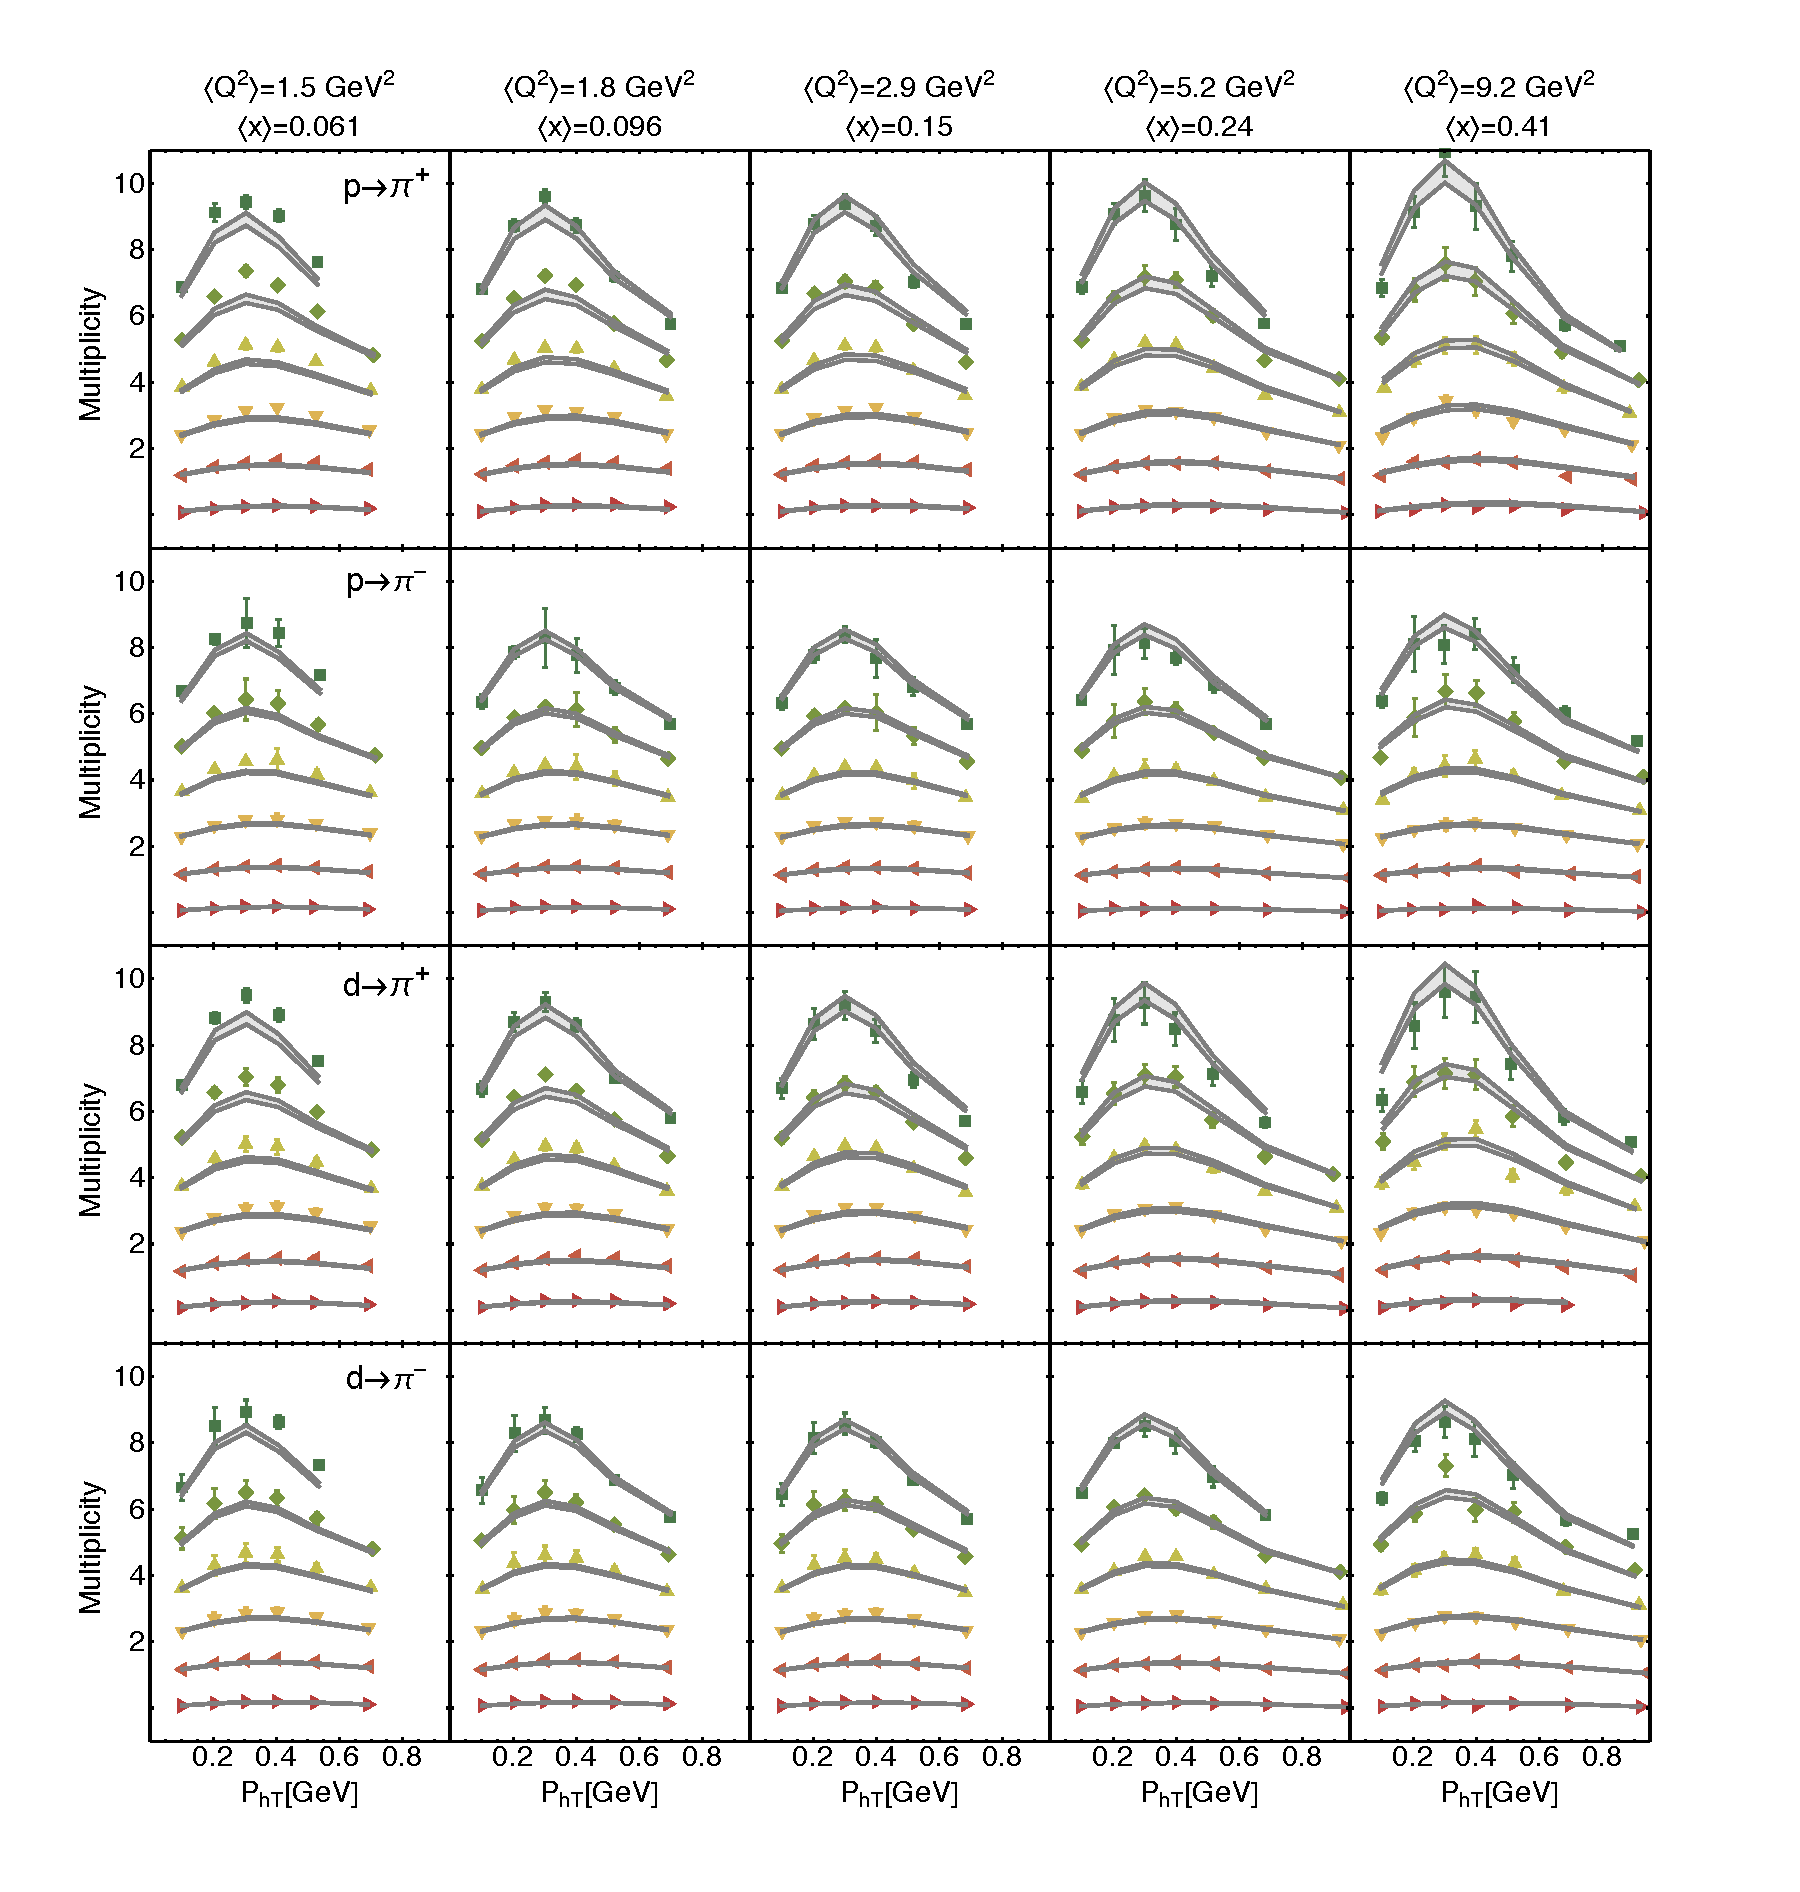
\includegraphics[width=0.90\textwidth]{plots/Hermes_Pions_SCIplot_flINDEP.pdf}
\end{center}
\caption{Hermes multiplicities for production of pions off a proton and a deuteron for different $\langle x \rangle$, $\langle z \rangle$, and $\langle Q^2 \rangle$ bins as a funciton of the transverse momentum of the dected hadron  $P_{hT}$.} 
\label{f:H_pions}
\end{figure}
%%%%%%%%%%%%%%%%%%%%%%%%%%%%%%%%%
\begin{figure}[h!]
\begin{center}
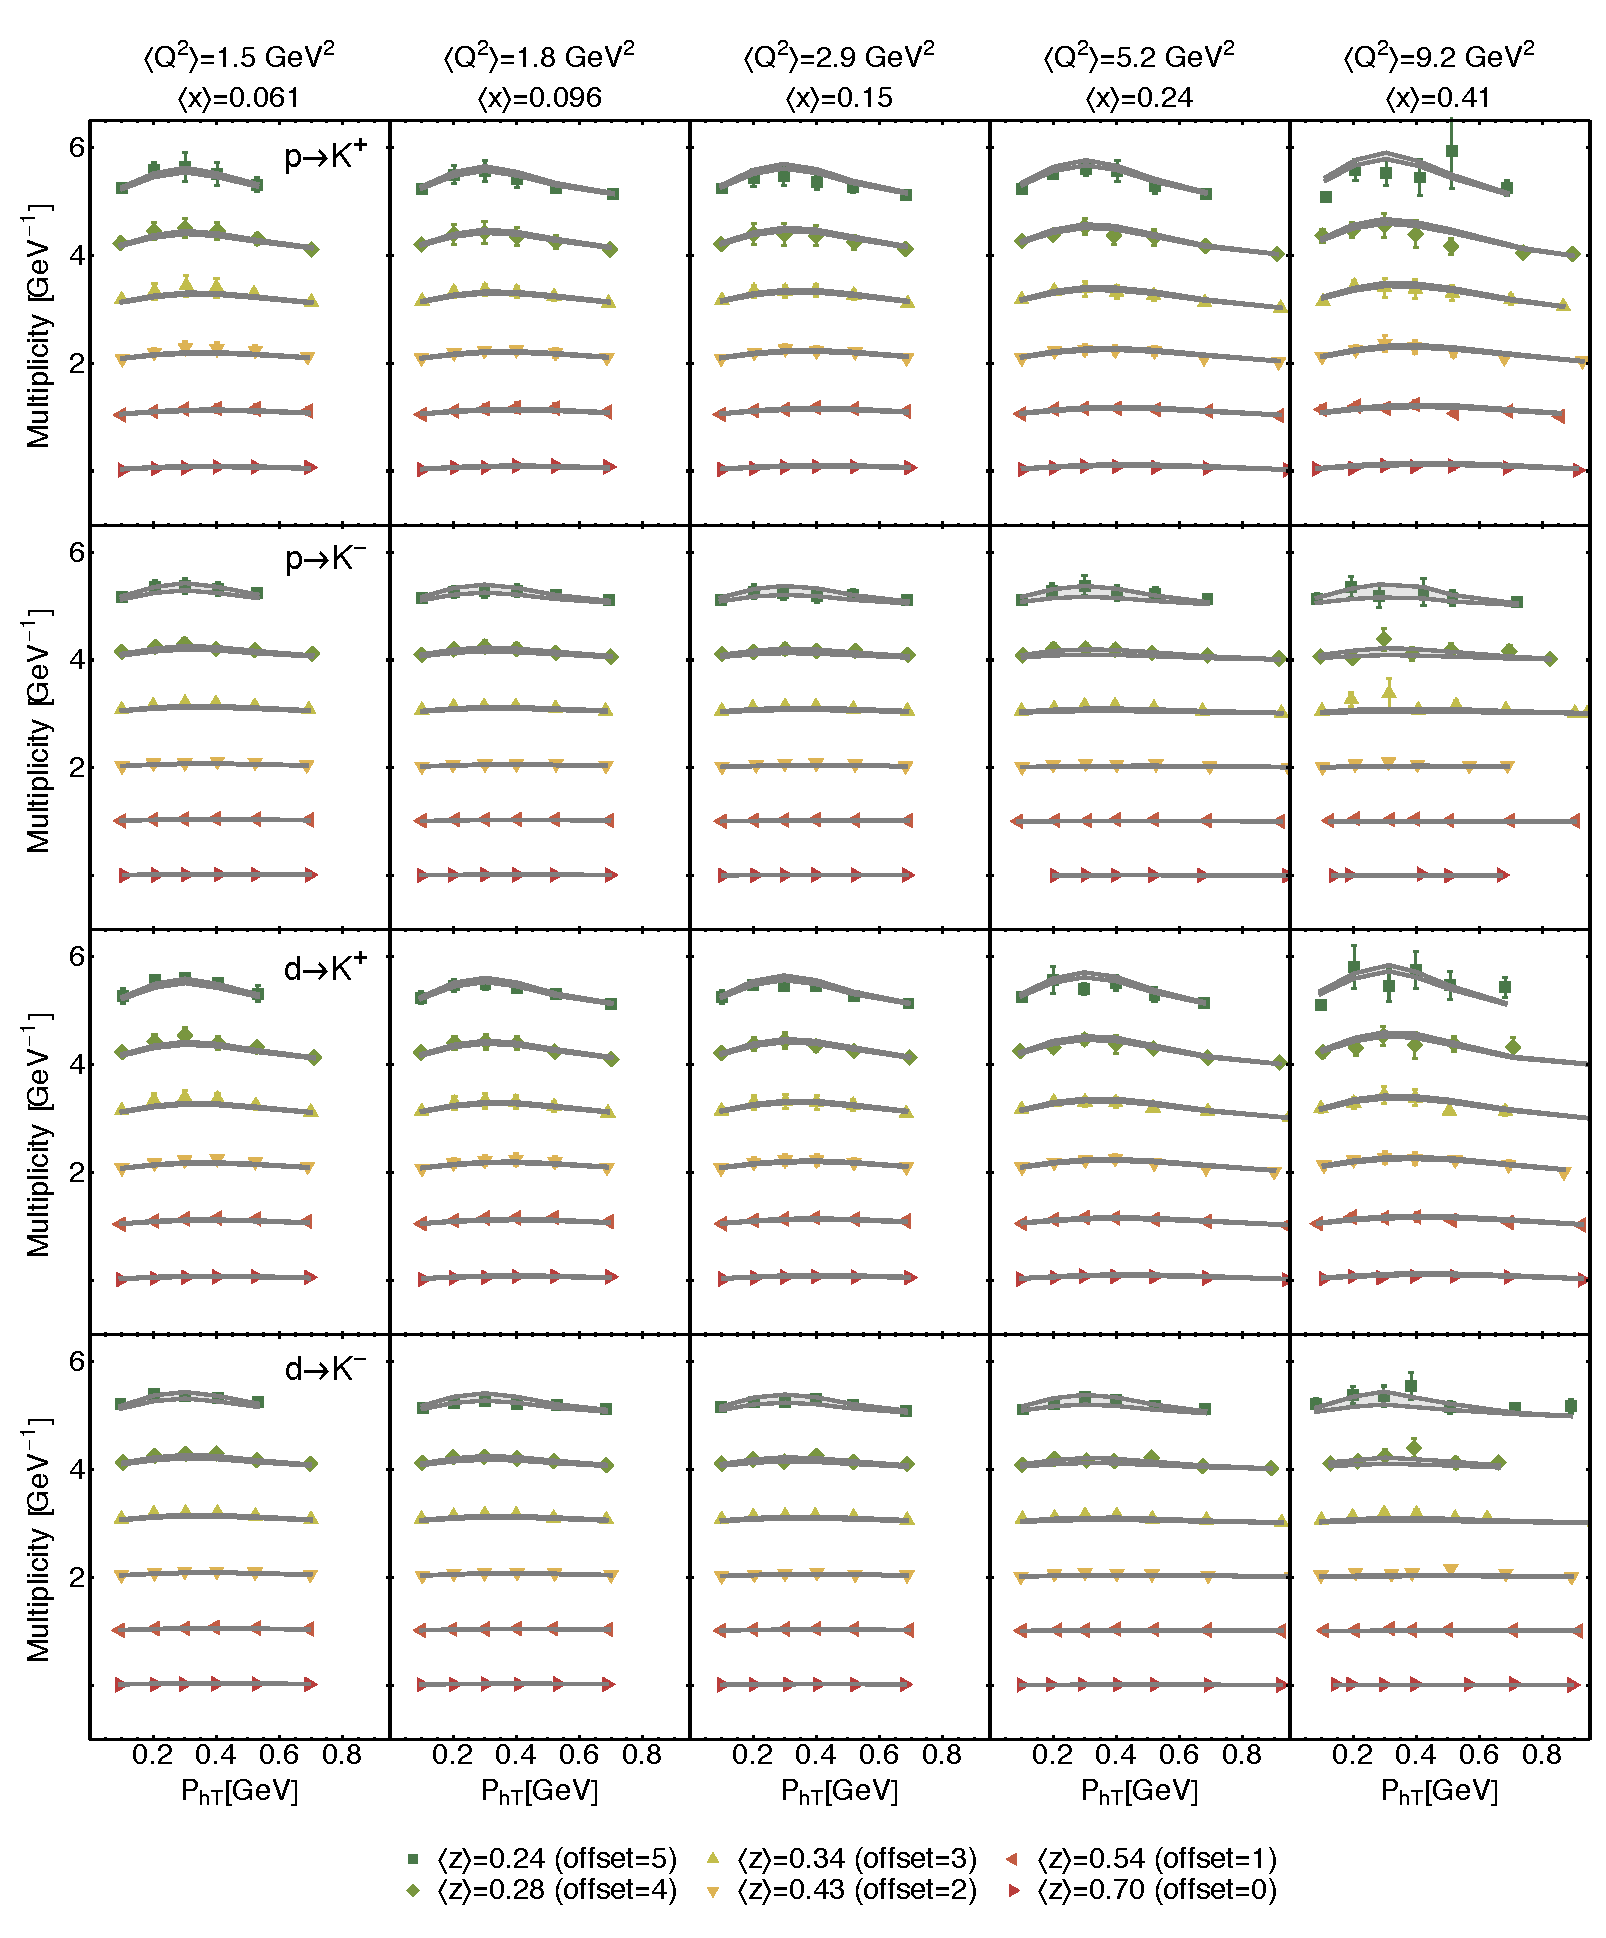
\includegraphics[width=0.90\textwidth]{plots/Hermes_Kaons_SCIplot_flINDEP.pdf}
\end{center}
\caption{Hermes multiplicities for production of kaons off a proton and a deuteron for different $\langle x \rangle$, $\langle z \rangle$, and $\langle Q^2 \rangle$ bins as a funciton of the transverse momentum of the dected hadron $P_{hT}$.} 
\label{f:H_kaons}
\end{figure}
%%%%%%%%%%%%%%%%%%%%%%%%%%%%%%%%%
\begin{figure}[h!]
\begin{center}
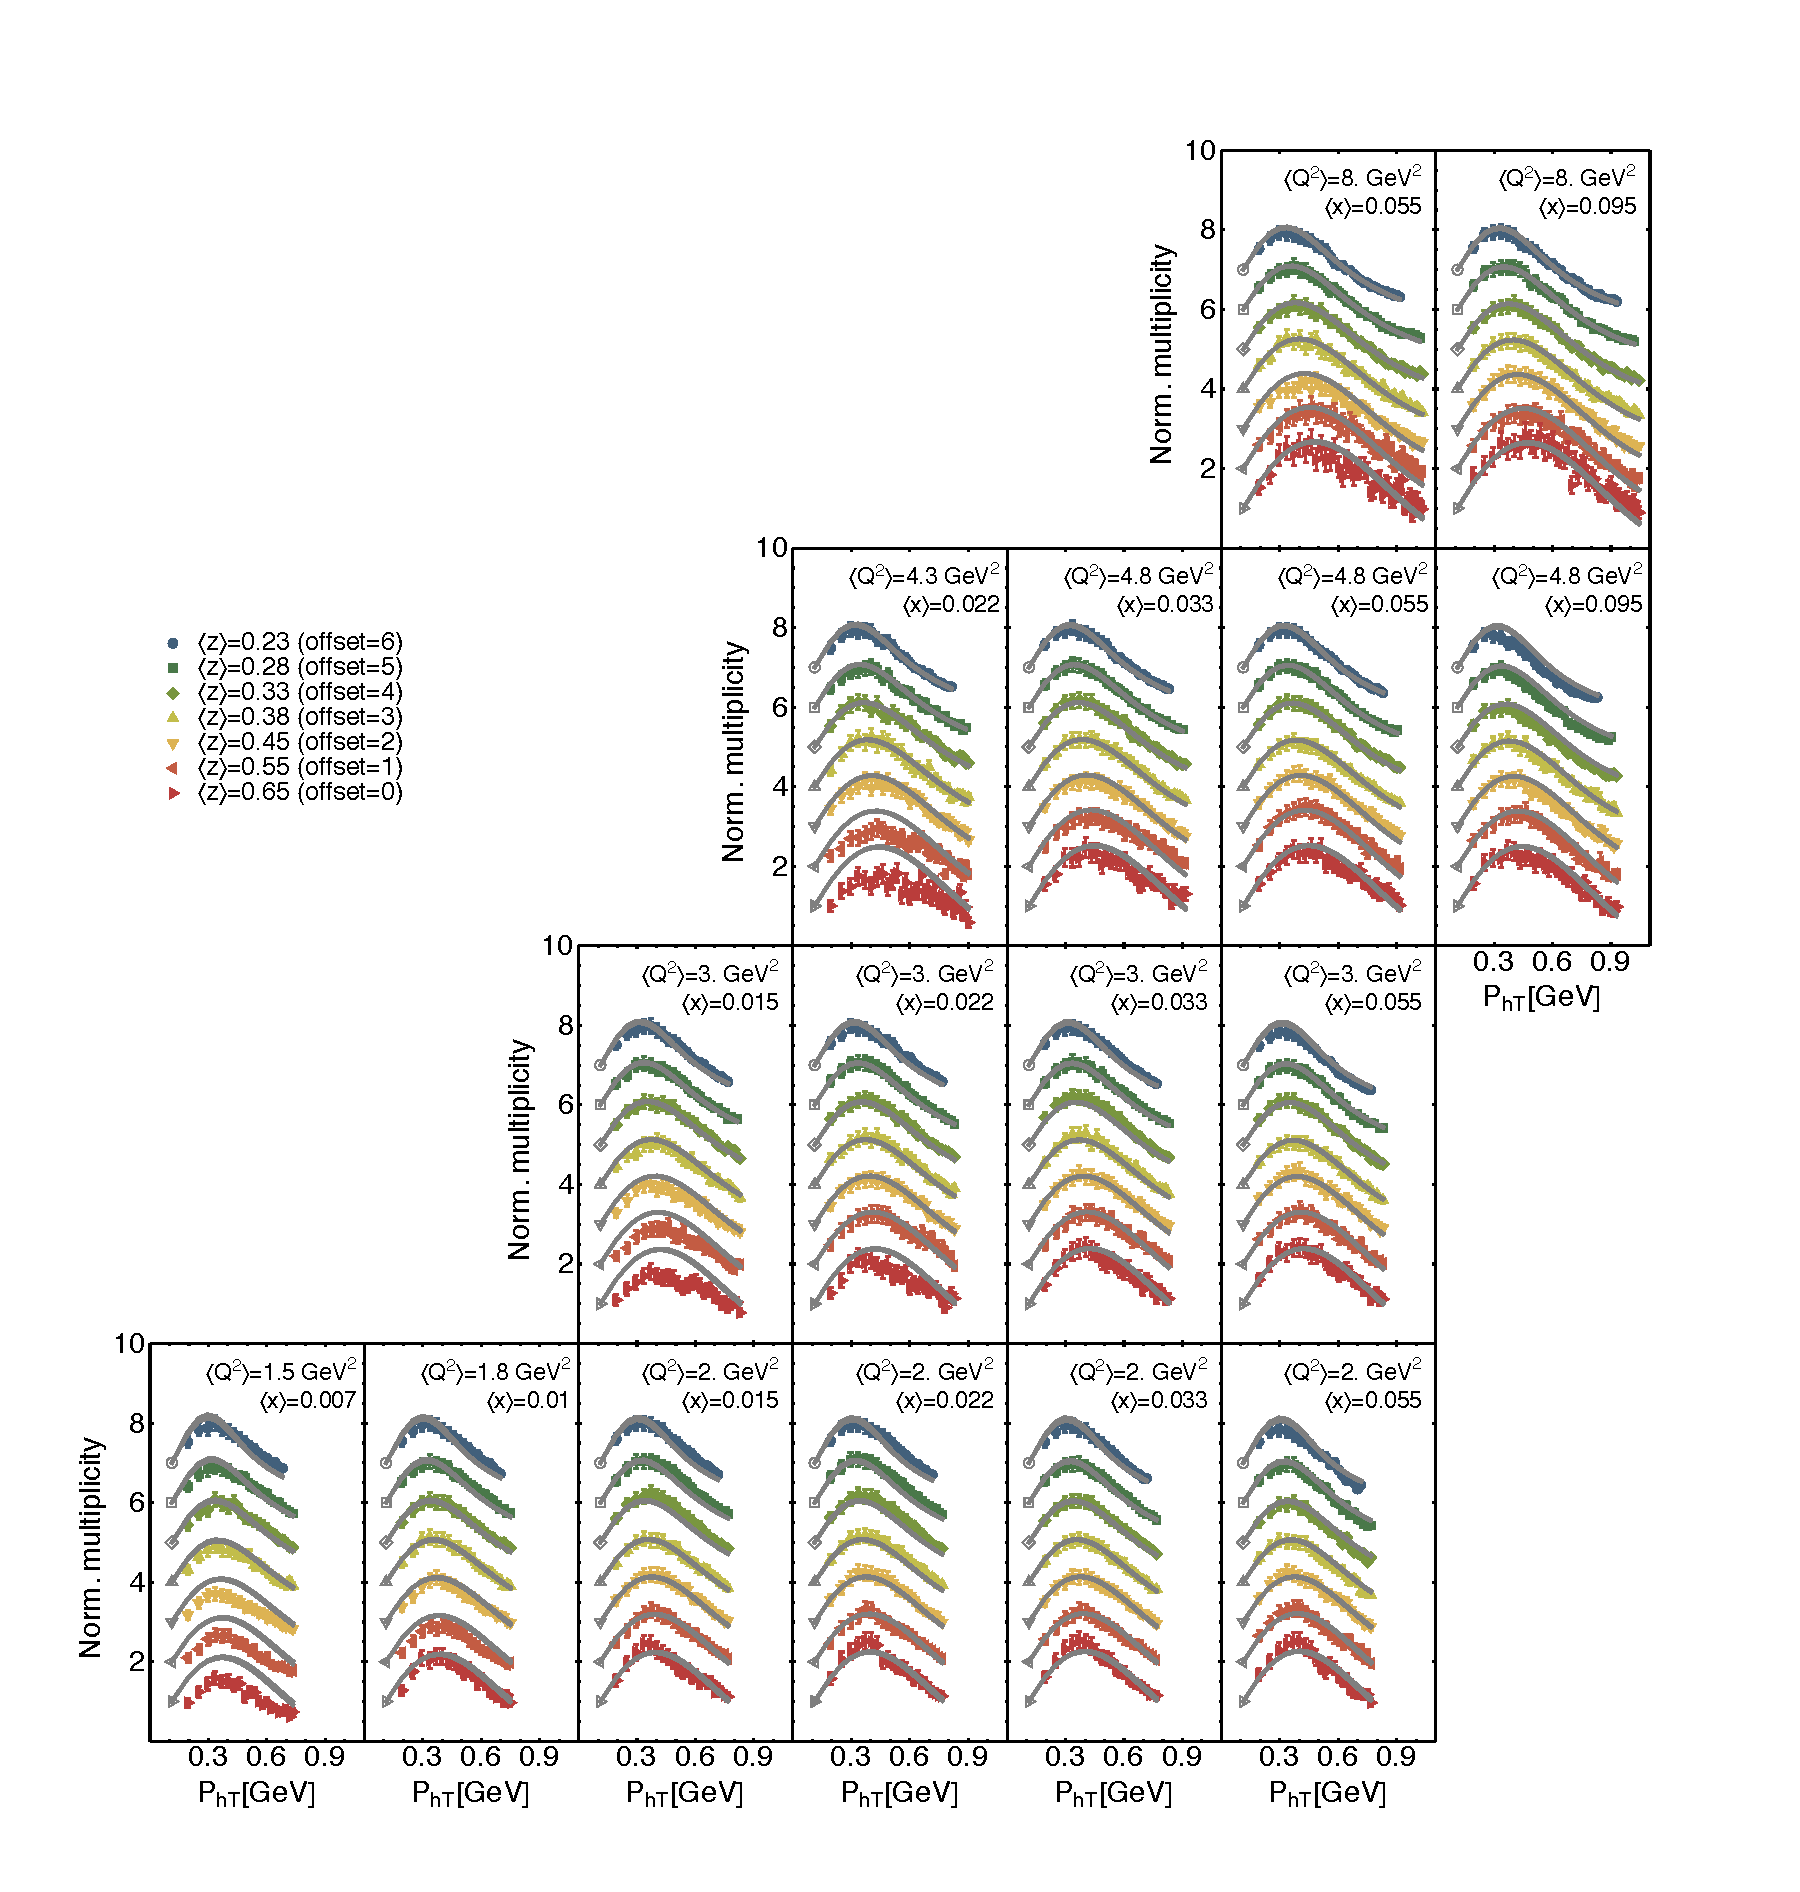
\includegraphics[width=\textwidth]{plots/COMPASS_SCIplot_flINDEP_Piminus.pdf}
\end{center}
\caption{Compass multiplicities for production of negative hadrons ($\pi^-$) off a deuteron for different $\langle x \rangle$, $\langle z \rangle$, and $\langle Q^2 \rangle$ bins as a funciton of the transverse momentum of the dected hadron  $P_{hT}$. Multiplicities are normalized to the first bin in $P_{hT}$ for each $\langle z \rangle$ value (see~\eqref{e:mult_norm}). For clarity, each $\langle z \rangle$  bin has been shifted by an offset indicated in the legend.} 
\label{f:C_pim}
\end{figure}
%%%%%%%%%%%%%%%%%%%%%%%%%%%%%%%%%
\begin{figure}[h!]
\begin{center}
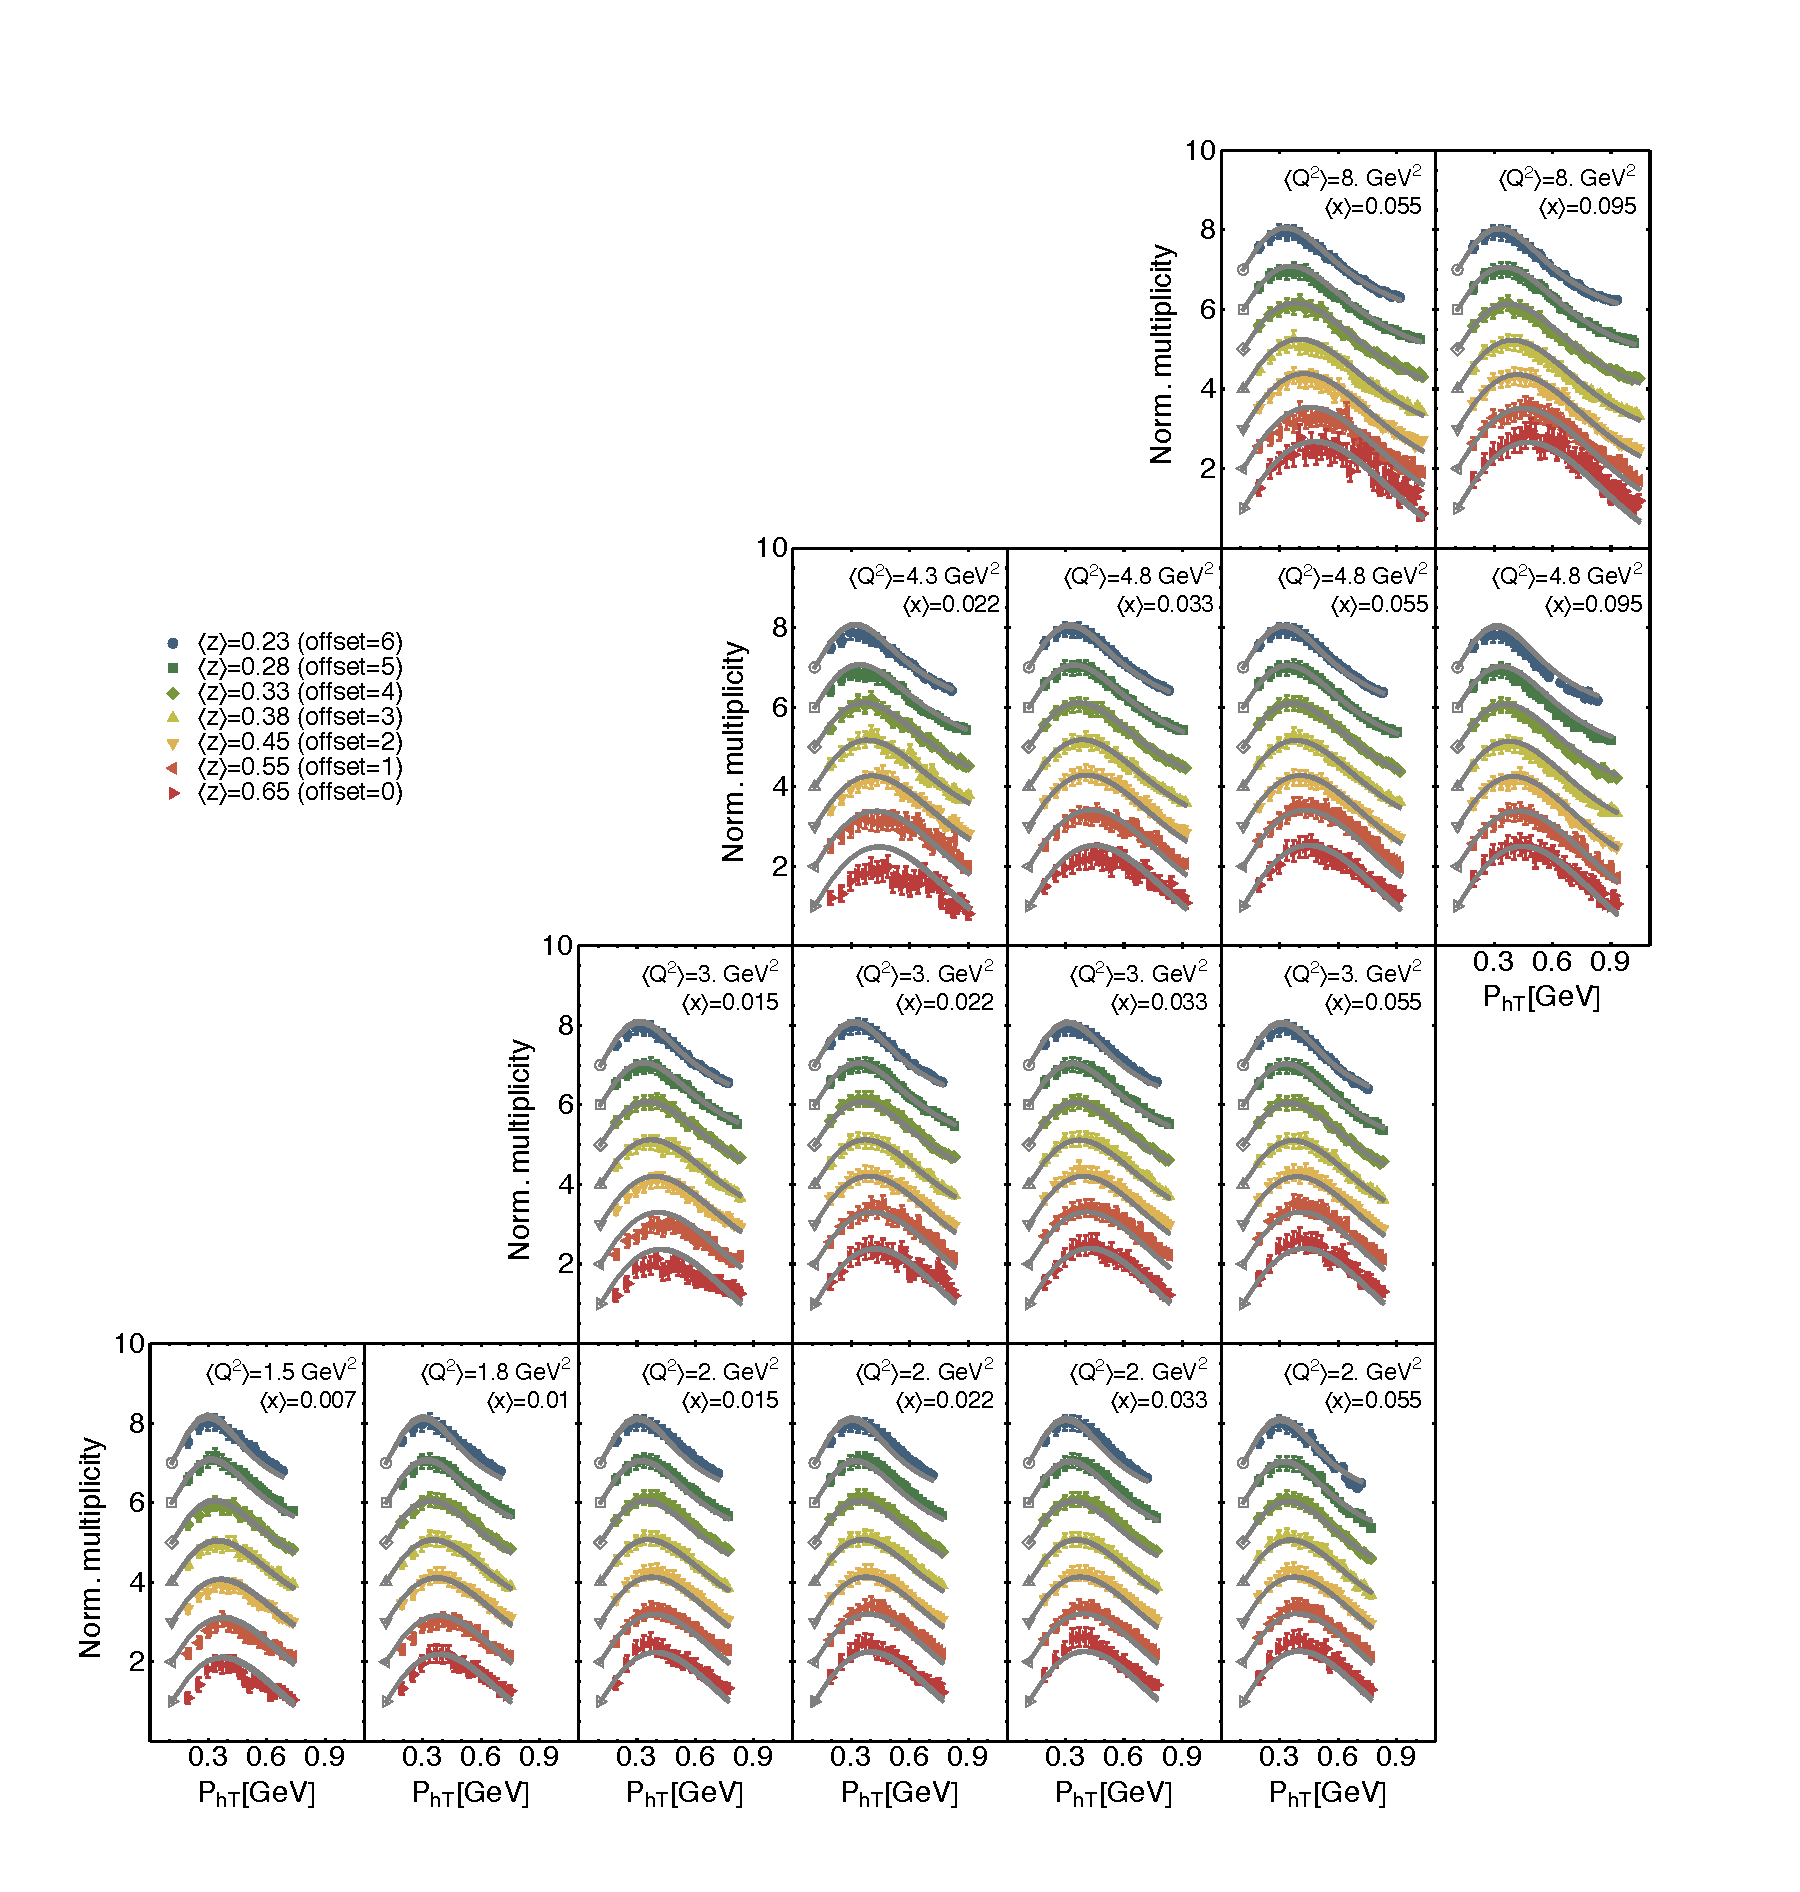
\includegraphics[width=\textwidth]{plots/COMPASS_SCIplot_flINDEP_Piplus.pdf}
\end{center}
\caption{Compass multiplicities for production of positive hadrons ($\pi^+$) off a deuteron for different $\langle x \rangle$, $\langle z \rangle$, and $\langle Q^2 \rangle$ bins as a funciton of the transverse momentum of the dected hadron $P_{hT}$. Multiplicities are normalized to the first bin in  $P_{hT}$ for each $\langle z \rangle$ value (see~\eqref{e:mult_norm}). For clarity, each $\langle z \rangle$  bin has been shifted by an offset indicated in the legend.} 
\label{f:C_pip}
\end{figure}
%%%%%%%%%%%%%%%%%%%%%%%%%%%%%%%%%





\subsubsection*{Drell-Yan processes}
\label{sss:DYZ_agreement}

%%% CHI2 VALUES %%%

The low energy Drell-Yan data collected by the E288 and E605 experiments at Fermilab have large error bands (see Fig.~\ref{f:DY_panel}). This is why the $\chi^2$ values in Tab.~\ref{t:fl_ind_chi2_DY} are rather low compared to the other data sets. 

The agreement is also good for $Z$ boson production, see Tab.~\ref{t:fl_ind_chi2_Z}. The statistics from Run-II is higher, which generates smaller experimental uncertainties and higher $\chi^2$, especially for the CDF experiment.
%%%%%%%%%%%%%% Tab. chi2 Drell-Yan low Q %%%%%%%%%%%%%%%%%%%%%%%%%%
\begin{table}[h!]
\begin{center}
%\newcommand{\m}{\hphantom{$-$}}
%\newcommand{\cc}[1]{\multicolumn{1}{c}{#1}}
\renewcommand{\tabcolsep}{0.4pc} % enlarge column spacing
\renewcommand{\arraystretch}{1.2} % enlarge line spacing
\begin{tabular}{|c|c|c|c|c|}
 \hline
 \hline
 ~                        &  E288 [200]    &  E288 [300]        &  E288 [400]          &  E605                \\
 \hline
 Points                   &      45      &   45             &       78           &     35               \\
 \hline
$ \chi^2  /$points      &  0.99        &    0.84           &       0.32
&   1.12     \\
\hline
\hline
\end{tabular}
\caption{Number of points analyzed and $\chi^2$ values for fixed-target Drell-Yan experiments at low energy. The labels in square brackets were introduced in Sec.~\ref{ss:dy}.}
\label{t:fl_ind_chi2_DY}
\end{center}
\end{table}
%%%%%%%%%%%%%% Tab. chi2 Z Tevatron %%%%%%%%%%%%%%%%%%%%%%%%%%
\begin{table}[h!]
\begin{center}
%\vskip 18pt
%\newcommand{\m}{\hphantom{$-$}}
%\newcommand{\cc}[1]{\multicolumn{1}{c}{#1}}
\renewcommand{\tabcolsep}{0.4pc} % enlarge column spacing
\renewcommand{\arraystretch}{1.2} % enlarge line spacing
\begin{tabular}{|c|c|c|c|c|}
 \hline
\hline
 ~                        & CDF Run I    &  D0 Run I        & CDF Run II        & D0 Run II      \\
 \hline
 Points                   &      31      &   14             &       37          &        8       \\
 \hline
$\chi^2 /$points      &  1.36        &    1.11           &       2.00         &   1.73     \\
\hline
\hline
\end{tabular}
\caption{Number of points analyzed and $\chi^2$ values for $Z$ boson production at Tevatron.}
\label{t:fl_ind_chi2_Z}
\end{center}
\end{table}
%%%%%%%%%%%%%%%%%%%%%%%%%%%%%%%%%%%%%%%%%%%%%%%%%%%%%%%%%%%%%%%



%%% FIGURES %%%

Fig.~\ref{f:DY_panel} displays the cross section for DY events differential with respect to the transverse momentum $q_T$ of the virtual photon, its invariant mass $Q^2$ and rapidity $y$.  
As for the case of SIDIS, the grey bands are the $68\%$ C.L. envelope of the 200 replicas of the fit function. The four panels represents different values for the rapidity $y$ or $x_F$ (see~\eqref{e:eta_xf}). In each panel, we have plots for different $Q^2$ values.
The lower is $Q$, the less points in $q_T$ we fit (see also Sec.~\ref{ss:dy}). 
The hard scale lies in the region $4.5 < \langle Q \rangle < 13.5$ GeV. This region is of particular importance, since these ``moderate'' $Q$ values are high enough to safely apply factorization without pollution from higher twist effects and from the very low $b_T$ region and, at the same time, low enough in order for the nonperturbative effects to not be shaded by transverse momentum resummation.
A visible effect of TMD evolution is the shift of the peak position to higher $q_T$ as $Q$ increases (effect visible in each panel in Fig.~\ref{f:DY_panel}). 
In Fig.~\ref{f:Z_qT} we compare the cross section differential with respect to the transverse momentum $q_T$ of the virtual $Z$ (namely Eq.~\eqref{e:dsigma_gZ} integrated over $\eta$) with data from CDF and D0 at Tevatron Run I and II. 
Due to the higher $Q = M_Z$, the range explored in $q_T$ is much larger compared to all the other observables considered. The tails of the distributions clearly deviate from a Gaussian behavior, as it is also evident in the bins at higher $Q^2$ in Fig.~\ref{f:DY_panel}. The band from the replica methodology in this case is much narrower, due to the reduced sensitivity to the intrinsic transverse momenta at $Q=M_Z$ and to the limited range of best-fit values for the parameter $g_2$, which controls soft-gluon emission. 
As an effect of TMD evolution, the peak shifts from $\sim 1$ GeV for Drell-Yan events in Fig.~\ref{f:DY_panel} to $\sim 5$ GeV in Fig.~\ref{f:Z_qT}. The position of the peak is affected both by the perturbative and the nonperturbative part of the Sudakov exponent (see Sec.~\ref{ss:TMDevo} and~\cite{Signori:2016lvd}).
Most of the contributions to the $\chi^2$ comes from normalization effects and not from the shape in $q_T$. 

%%%%%%%%%%%%%%%%%%%%%%%%%%%%%%%%%%
\begin{figure}[h!]
\centering
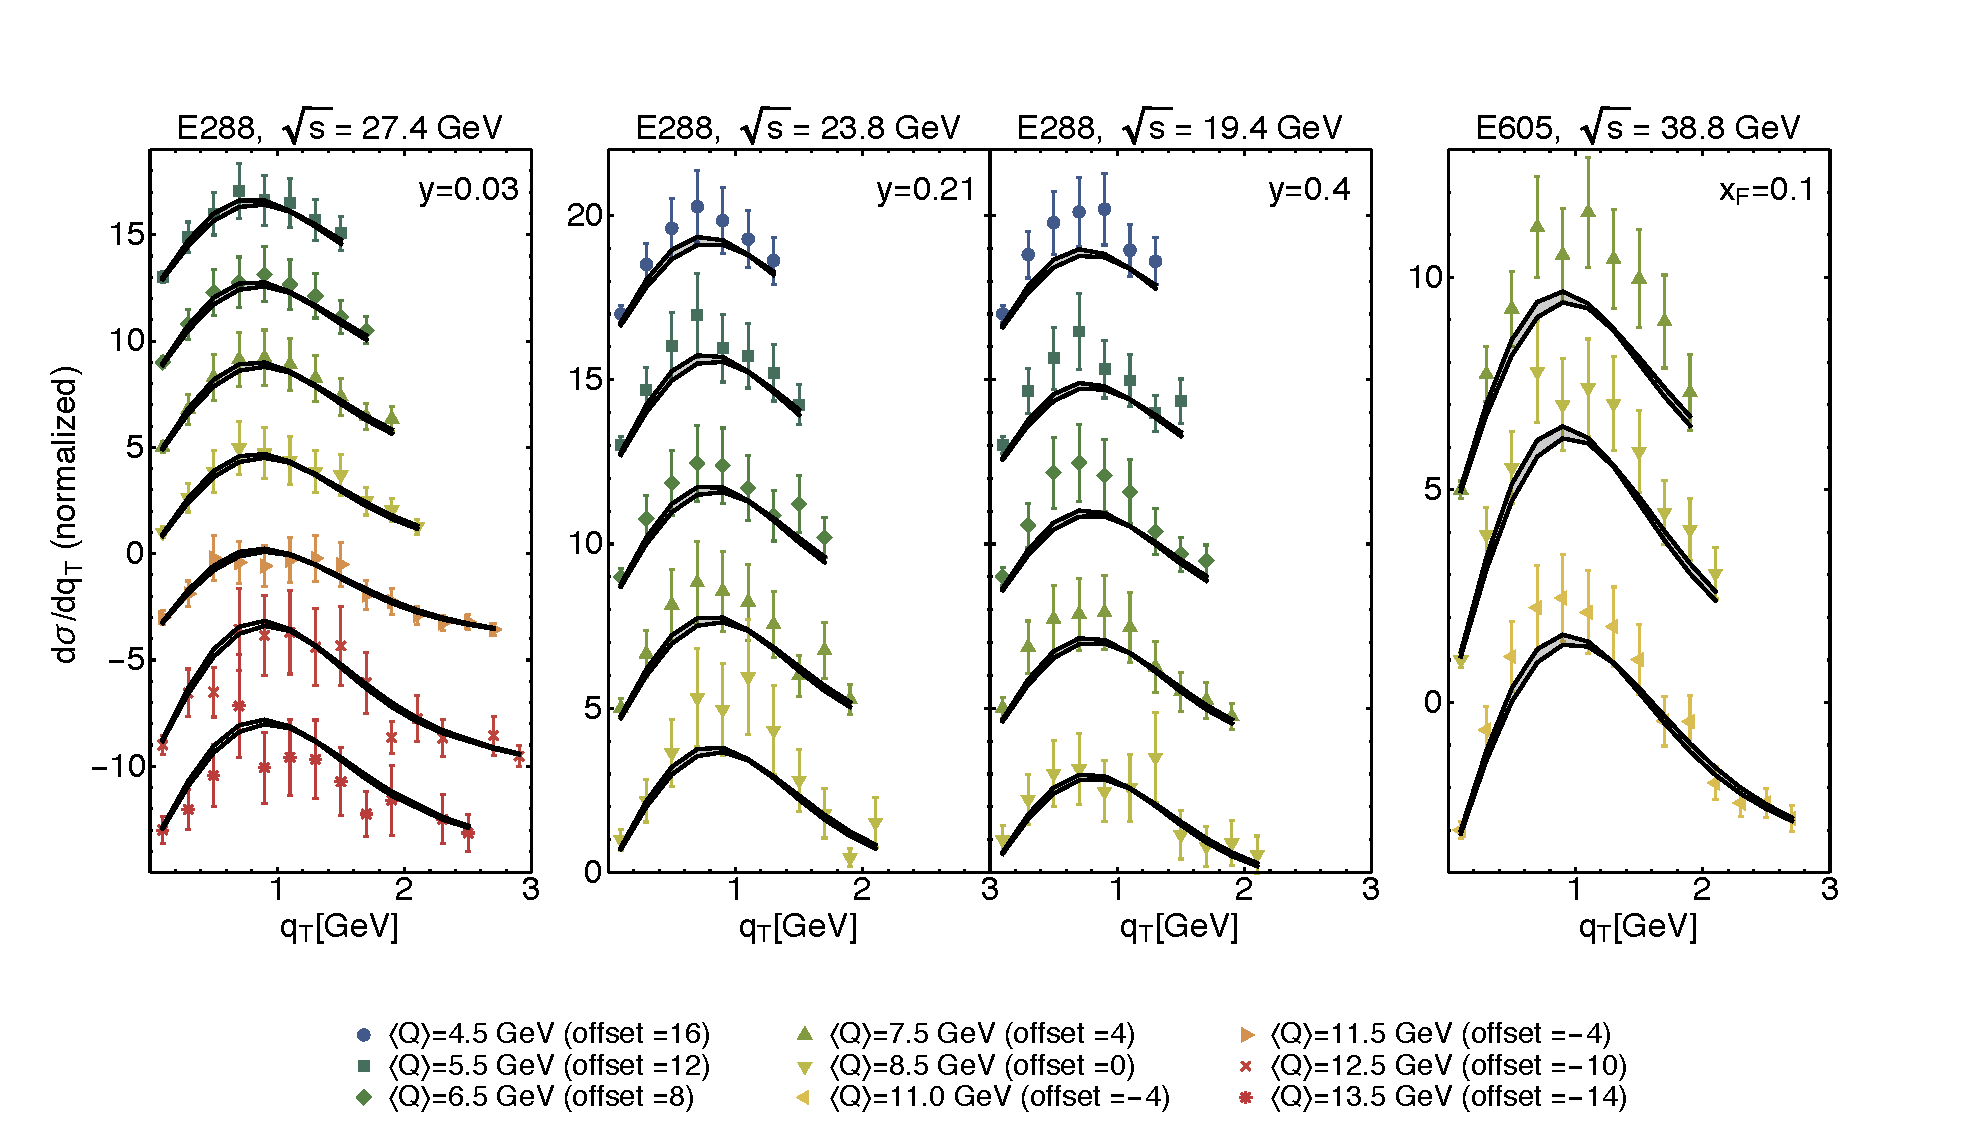
\includegraphics[width=0.95\textwidth]{plots/DY_SCIplot_flINDEP.pdf}
\caption{Drell-Yan differential cross section for different experiments and different values of $\sqrt{s}$ and for different $\langle Q \rangle$ bins. For clarity, each $\langle Q \rangle$  bin has been shifted by an offset indicated in the legend. \textcolor{red}{AS: is the cross section differential in $Q^2$ and rapidity $\eta$ (or $y$?) ``Normalized''=?}}
\label{f:DY_panel}
\end{figure}
%%%%%%%%%%%%%%%%%%%%%%%%%%%%%%%%%
\begin{figure}[h!]
\begin{center}
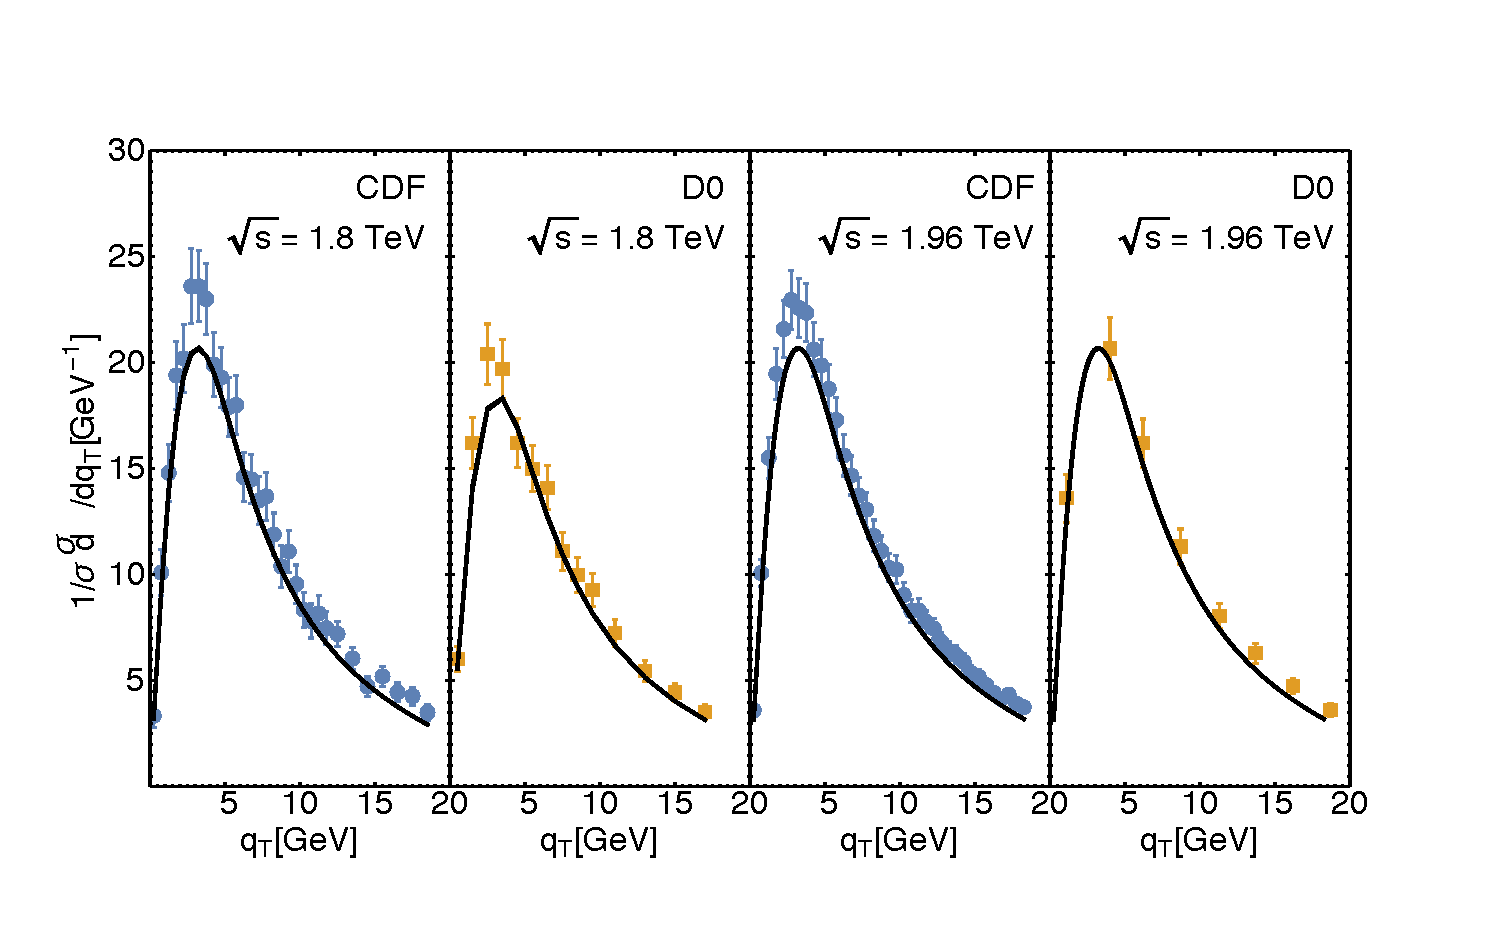
\includegraphics[width=0.95\textwidth]{plots/Z_SCIplot_flINDEP.pdf}
\end{center}
\caption{Cross section differential with respect to the transverse momentum $q_T$ of a $Z$ boson produced from $p\bar{p}$ collisions at Tevatron. The four panels refer to different experiments (CDF and D$0$) with two different values for the center-of-mass energy ($\sqrt{s} = 1.8$ TeV and $\sqrt{s}=1.96$ TeV). In this case the band is narrow due to the narrow range for the best-fit values of $g_2$.} 
\label{f:Z_qT}
\end{figure}
%%%%%%%%%%%%%%%%%%%%%%%%%%%%%%%%%








%========================================================
\subsection{Transverse momentum dependence at 1 GeV}
\label{ss:bestfit_TMDs}

%% separation in bT space
The variables $\bb_{\rm min}$ and $\bb_{\rm max}$ delimit the range in $b_T$ where transverse momentum resummation is computed perturbatively. $\bb_{\rm max}$ allows to avoid the Landau pole and $\bb_{\rm min}$ allows to recover correctly the high transverse momentum limit of the cross section (see also Sec.~\ref{ss:TMDevo}).
The parameter $g_2$ which enters the nonperturbative Sudakov exponent quantifies the amount of soft gluons radiated.
As already detailed in Sec.~\ref{ss:TMDevo}, in this work we fix the value for $\bb_{\rm min}$ and $\bb_{\rm max}$ in such a way that at $Q=1$ GeV the unpolarized TMDs coincide with their nonperturbative input. $g_2$, instead, is a fit parameter.

Tab.~\ref{t:fl_ind_parcommon} summarizes the chosen values of $\bb_{\rm min}$, $\bb_{\rm max}$ and the best-fit value for $g_2$. The latter is given as an average with $68\%$ C.L. uncertainty computed over the set of 200 replicas. A similar value ($g_2 = 0.184 \pm 0.018$) was found in~\cite{Konychev:2005iy}.
We stress here that a prescription involving both $\bb_{\text{min}}$ and $\bb_{\text{max}}$ is equivalent to request $\mu_{\bar{b^*}}^2 < Q^2 \equiv \mu^2$ for all $b_T$ values in~\eqref{e:Sudakov}. This requirement turns out to be crucial in order to fit SIDIS data with TMD evolution and without a $Y$-term.

%% best fit values and transverse momenta
Tab.~\ref{t:fl_ind_par_TMD} collects the best-fit values of parameters in the nonperturbative part of the TMDs at $Q=1$ GeV (see~\eqref{e:f1NP} and~\eqref{e:D1NP}); we give the average value over the full set of replicas and the standard deviation based on a $68\%$ C.L. (see Sec.~\ref{ss:replica_method}). 
We also compare these values with the best-values from replica $105$.

Keeping in mind that $\big \langle \hat{\bm{k}}_{\T}^2 \big \rangle = \big \langle \bm{k}_{\T}^2 \big \rangle (x=0.1)$ and  $\big \langle \hat{\bm{P}}_{\perp}^2 \big \rangle = \big \langle \bm{P}_{\perp}^2 \big \rangle (z=0.5)$, we note that the average value of $\big \langle \hat{\bm{k}}_{\T}^2 \big \rangle$ is similar to and compatible within error bands with the value given in~\cite{Signori:2013mda} for the flavor-independent scenario. The value of $\big \langle \hat{\bm{P}}_{\perp}^2 \big \rangle$ is larger but still compatible with the same quantity given in~\cite{Signori:2013mda}. Comparisons between the two fits are anyway delicate, since here we rely on a modified Gaussian ansatz, see~\eqref{e:f1NPk} and~\eqref{e:D1NPk}.
Fig.~\ref{f:kT2_vs_PT2} is useful to compare diffferent extractions of partonic transverse momenta. The red area corresponds to the $68\%$ confidence region for $\{ \big \langle \hat{\bm{k}}_{\T}^2 \big \rangle$, $\big \langle \hat{\bm{P}}_{\perp}^2 \big \rangle \}$ pairs. Each black dot is an outcome of one fit (replica). The same applies to the orange region and its black dots, related to the flavor-independent analysis in~\cite{Signori:2013mda}. All the other points are related to different extractions and the color coding is described in the caption of Fig.~\ref{f:kT2_vs_PT2}. 
From the orange region (fit of SIDIS at \hermes only) a strong anticorrelation between the transverse momenta is evident. 
The inclusion of Drell-Yan and $Z$ production data adds physical information about the nonperturbative structure of  $f_1(x,k_\perp^2)$. This significantly reduces the spread in $\big \langle \hat{\bm{k}}_{\T}^2 \big \rangle$ and the correlation with $\big \langle \hat{\bm{P}}_{\perp}^2 \big \rangle$ (see the red region). 
The inclusion of \compass data, instead, determines a shift of the points and reduces the spread for $\big \langle \hat{\bm{P}}_{\perp}^2 \big \rangle$ values. 
These are important features of the fit and we should aim at including $e^+e^-$ data too to further reduce the correlation. Ideally in a global fit we will reach the lowest degree of correlation possible.  
When comparing different extractions, it is important to keep in mind that the intrinsic transverse momentum always depends on the scheme used to implement TMD evolution and its accuracy. 

% kinematic behavior of T.M. and correlations
Tab.~\ref{t:fl_ind_par_TMD} also presents the best-fit values for parameters shaping the kinematic dependence of $\big \langle \bm{k}_{\T}^2 \big \rangle (x)$, $\big \langle \bm{P}_{\perp}^2 \big \rangle (z)$, $\big \langle \bm{P}{\perp}^{\prime 2} \big \rangle (z)$ (see~\eqref{e:kT2_kin} and~\eqref{e:PT2_kin}). Since the values are all positive the average square transverse momenta cannot diverge in the limits $x,z \to 0$ or $1$. 
The kinematic dependence is shown in Fig.~\ref{f:avmomenta_68CL} (a) for $\big \langle \bm{k}_{\T}^2 \big \rangle (x)$ and Fig.~\ref{f:avmomenta_68CL} (b) for $\big \langle \bm{P}_{\perp}^2 \big \rangle (z)$. The plot for $\big \langle \bm{P}{\perp}^{\prime 2} \big \rangle (z)$ is identical to Fig.~\ref{f:avmomenta_68CL} (b) apart from a normalization factor. 
The pink bands are computed as the $68\%$ C.L.  envelope of the full sets of curves from the 200 replicas. Comparison with other extractions are presented and the legenda is detailed in the caption of Fig.~\ref{f:kT2_vs_PT2}.\\

\textcolor{red}{AS: shall we add plots for $f_1(x,k_\perp^2)$ and $D_1(z,P_\perp^2)$ to illustrate their shape at $Q=1$ GeV in momentum space?}
%%%%%%%%%%%%%%%% Tab. common parameters %%%%%%%%%%%%%%%%%%%%%%%%%%
\begin{table}[h!]
\small
  \centering
  \begin{tabular}{|c|c|c|c|}
\hline
\hline
%  \multicolumn{4}{|c|}{Parameters for TMD PDFs} \\
%  \hline
%  \hline
&$\bb_{\rm max}$ [GeV$^{-1}$] & $\bb_{\rm min}$ [GeV$^{-1}$] &  $g_2$ {[GeV$^2$]} 
 \\ 
& (fixed)     & (fixed)   &                            \\
\hline
All replicas & $2 e^{-\gamma_E}[/$GeV]& $2 e^{-\gamma_E}/Q$  & $0.13 \pm 0.01$  \\
\hline
Replica 105 &  $2 e^{-\gamma_E}[/$GeV]& $2 e^{-\gamma_E}/Q$  & $0.128$  \\
\hline
\hline
\end{tabular}
\caption{Values of parameters common to TMD PDFs and TMD FFs.}
\label{t:fl_ind_parcommon}
\end{table}
%%%%%%%%%%%%%%% Tab. results paramters TMDs %%%%%%%%%%%%%%%%%%%%%%
\begin{table}[h!]
\small
  \centering
  \begin{tabular}{|c||c|c|c|c|c|c|}
\hline
\hline
%  \multicolumn{4}{|c|}{Parameters for TMD PDFs} \\
%  \hline
%  \hline
TMD PDFs&  $\big \langle \hat{\bm{k}}_{\T}^2 \big \rangle$ 
& $\alpha$ & $\sigma$ & & $\lambda$ &  
 \\ 
        & {[GeV$^2$]}                               &
       &      &  &{[GeV$^{-2}$]} & \\
\hline
All replicas &  $0.28\pm 0.06$ & $2.95\pm 0.05$ & $0.17\pm 0.02$ & 
                & $0.86\pm 0.78$ & 
\\
\hline
Replica 105  &  $0.285$ & $2.98$ & $0.173$ & & $0.39$ & \\
\hline
\hline
TMD FFs&  $\big \langle \hat{\bm{P}}_{\perp}^2 \big \rangle$ &
$\beta$ & $\delta$ & $\gamma$ & $\lambda_F$ & $\big \langle
\hat{\bm{P}}_{\perp}^{\prime 2} \big \rangle$
 \\ 
        & {[GeV$^2$]} &            &        & &{[GeV$^{-2}$]} &{[GeV$^2$]}    \\
\hline
All replicas & $0.21\pm 0.02$ & $1.65\pm 0.49$ & $2.28\pm 0.46$ & $0.14\pm 0.07$ &
$5.50\pm 1.23$ & $0.13\pm 0.01$ \\
\hline
Replica 105   &  
 $0.212$ & $2.10$ & $2.52$ & $0.094$ & $5.29$ & $0.135$ \\
\hline
\hline
\end{tabular}
\caption{68\% confidence intervals of best-fit values for parametrizations of TMDs at $Q=1$ GeV.}
\label{t:fl_ind_par_TMD}
\end{table}
%%%%%%%%%%%%%%%%%%%%%%%%%%%%%%%%%%%%%%%%%%%%%%%%%%%%%%%%%%%
%%%%%%%%%%%%%%%%%%%%%%%%%%%%%%%%%
\begin{figure}[h!]
\begin{center}
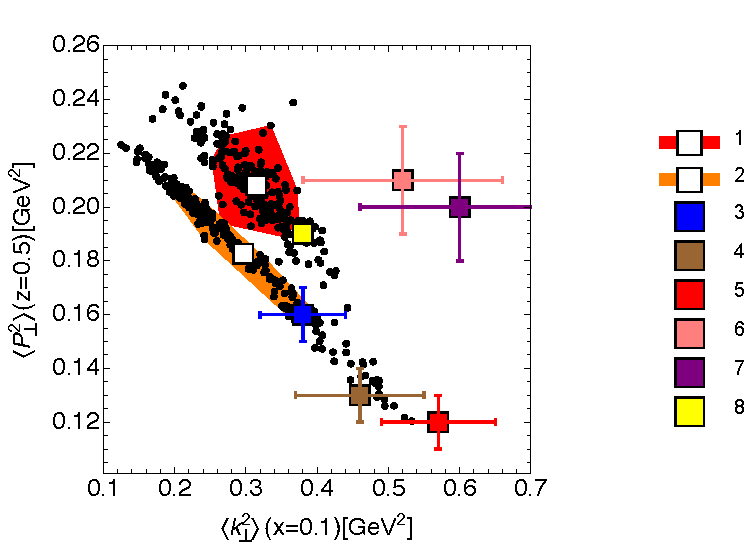
\includegraphics[width=0.60\textwidth]{plots/kT2_PT2_flav_indep}
\end{center}
\caption{Correlation between transverse momenta in TMD FFs, $\langle P_\perp^2 \rangle(z=0.5)$, and in TMD PDFs, $\langle k_\perp^2 \rangle(x=0.1)$, in different phenomenological extractions. 
The red region is the $68\%$ C.L. area explored in this fit (1-red). The white boxes represent the average values over the replicas for the transverse momenta. 
The other extractions are: (2-orange)~\cite{Signori:2013mda}, (3-blue)~\cite{Schweitzer:2010tt}, (4-brown)~\cite{Anselmino:2013lza} for \hermes data, (5-red point)~\cite{Anselmino:2013lza} for \hermes data at high $z$, (6-pink)~\cite{Anselmino:2013lza} for normalized \compass data, (7-purple)~\cite{Anselmino:2013lza} for normalized \compass data at high $z$, (8-yellow)~\cite{Echevarria:2014xaa}.  
For more details, such as the value of the input scale for the TMDs, see the respective references.} 
\label{f:kT2_vs_PT2}
\end{figure}
%%%%%%%%%%%%%%%%%%%%%%%%%%%%%%%%%
%\begin{figure}[h!]
%\centering
%\begin{tabular}{ccc}
%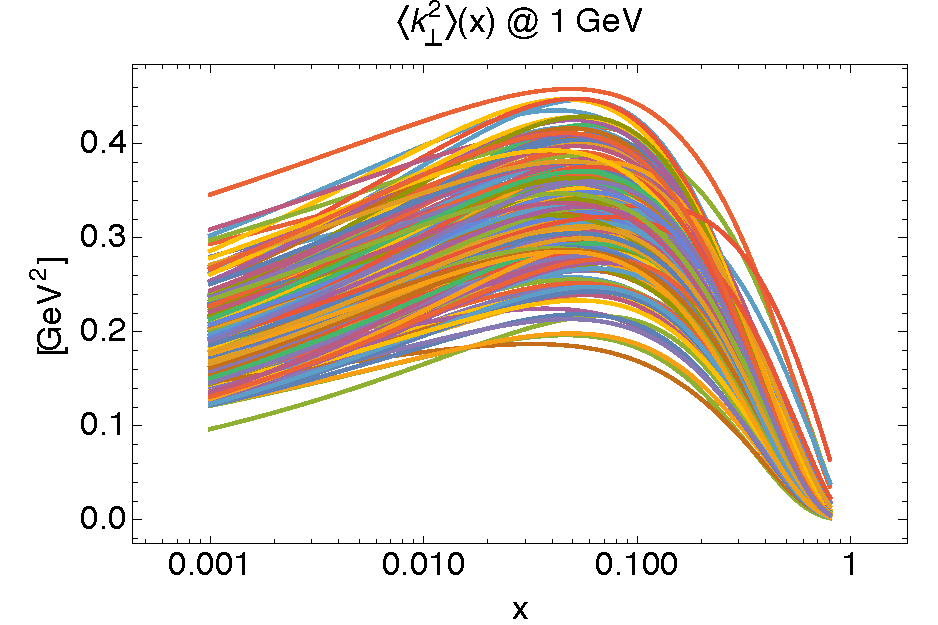
\includegraphics[width=0.40\textwidth]{plots/kT2av_curves_at1GeV_flINDEP.pdf}
%&\hspace{0.001cm}
%&
%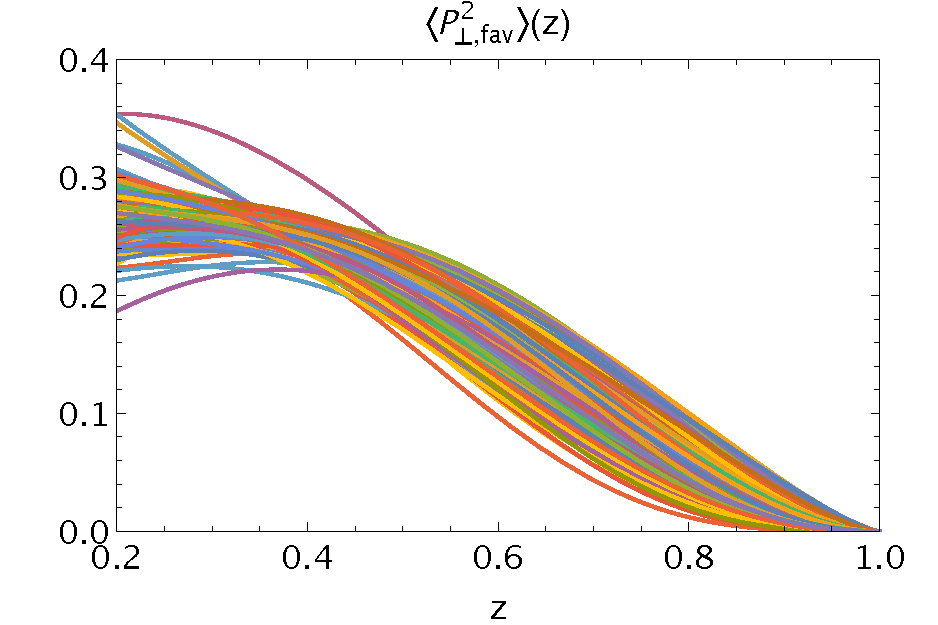
\includegraphics[width=0.40\textwidth]{plots/PT2av_curves_at1GeV_flINDEP.pdf}
%\\
%(a) && (b)
%\end{tabular}
%\caption{write the caption here (a) and another here (b).}
%\label{f:avmomenta_all_rep}
%\end{figure}
%%%%%%%%%%%%%%%%%%%%%%%%%%%%%%%%%
\begin{figure}[h!]
\centering
\begin{tabular}{ccc}
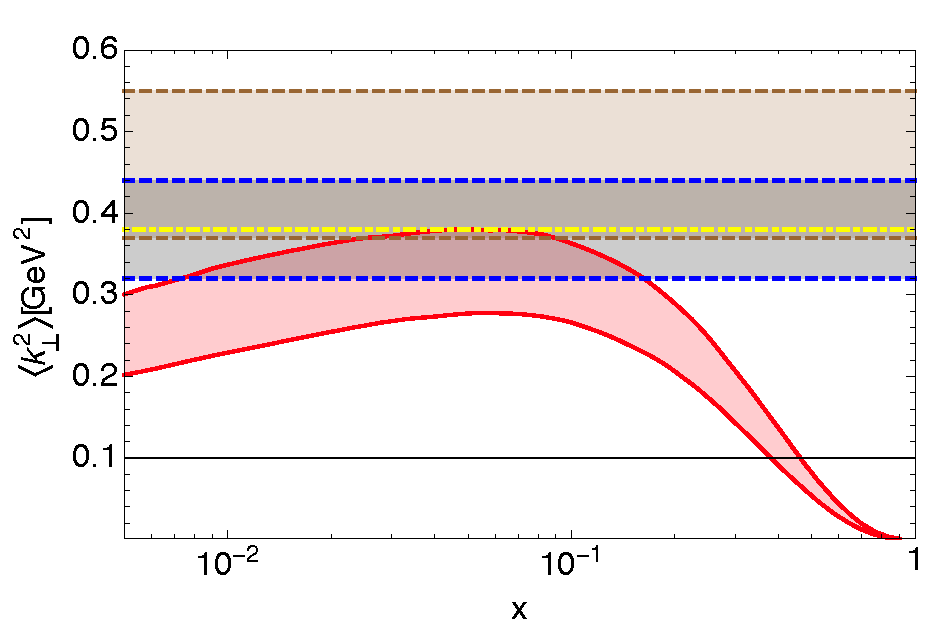
\includegraphics[width=0.40\textwidth]{plots/kT2av_Compare_with_other_extractions_flINDEP.pdf}
&\hspace{0.001cm}
&
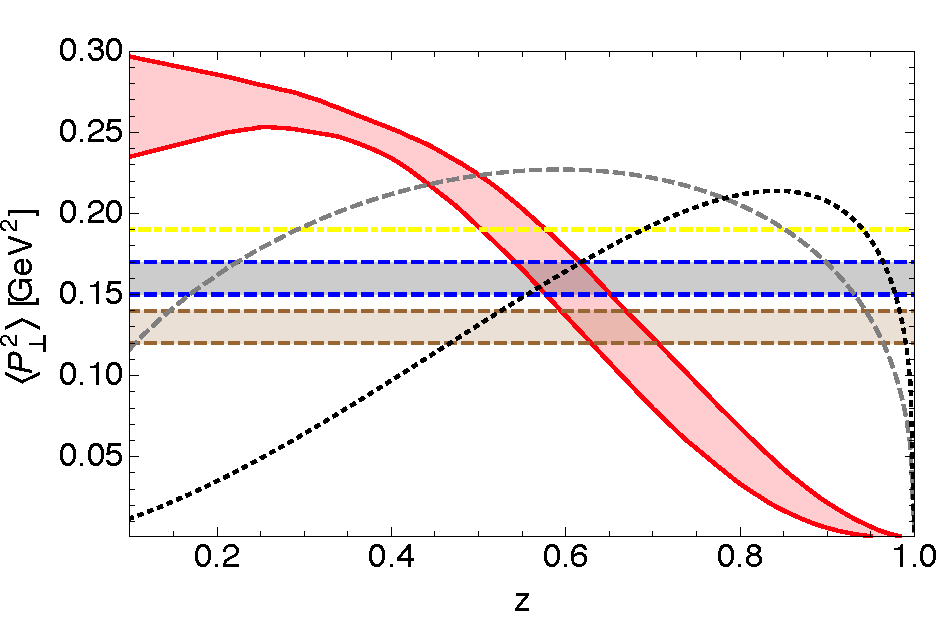
\includegraphics[width=0.40\textwidth]{plots/PT2av_Compare_with_other_extractions_flINDEP.pdf}
\\
(a) && (b)
\end{tabular}
\caption{Kinematic dependence of $\big \langle \bm{k}_{\T}^2 \big \rangle (x)$ (a) and of $\big \langle \bm{P}_{\perp}^2 \big \rangle (z)$ (b). The bands are the $68\%$ C.L. envelope of the full sets of best-fit curves. Comparisons with other extractions are displayed. Color coding is the same as in Fig.~\ref{f:kT2_vs_PT2}.  In (b) the grey-dashed curve refers to the parametrization used in GMCtrans~\cite{gmctrans} and the black-dashed curve refers to~\cite{Boglione:1999pz}. }
\label{f:avmomenta_68CL}
\end{figure}
%%%%%%%%%%%%%%%%%%%%%%%%%%%%%%%%%


%=======================================================
\subsection{Tests on replica 105}
\label{ss:replica105}

In this subsection we have a closer look at the results of the fit to replica 105, which, as discussed above, is one of the most representative of the two hundred fits performed in our analysis. The corresponding $\chi^2/$d.o.f.~is 1.51. We note that if we normalize \hermes data to the value of the first bin in $P_{hT}$ as we did for \compass data, the global  $\chi^2/$d.o.f.~immediately reduces to 1.27, without performing any new minimization. The partial $\chi^2$ for the different SIDIS processes measured at \hermes are shown in Table~\ref{t:replica105-hermes}.

%%%%%%%%%%%%%% Tab. chi2 SIDIS off deuteron %%%%%%%%%%%%%%%%%%%%%%%%%%
\begin{table}[h!]
\begin{center}
\begin{tabular}{|c|c|c|c|c|c|c|c|c|}
 \hline
\hline
%  & HERMES & HERMES & HERMES & HERMES  & HERMES & HERMES & HERMES & HERMES \\
 ~     &  $p \to \pi^+$    &   $p \to \pi^-$    &  $p \to K^+$    &   $p \to K^-$       &  $D \to \pi^+$    &   $D \to \pi^-$    &  $D \to K^+$    &   $D \to K^-$                \\
\hline
 Original   &  5.18 &  2.67 & 0.75  & 0.78      &  3.63 &  2.31 & 1.12  & 2.27    \\
 \hline
%$\chi^2$ &4.24 & 3.49 & 0.63 & 1.00                \\
Normalized  &  1.94 &  1.13 &  0.57 & 0.29 & 1.59  & 0.80 & 0.47 & 0.97  \\            
 \hline
 \hline
\end{tabular}
\caption{$\chi^2$/d.o.f.\ for \hermes data with and without normalization to the value of the first bin in $P_{hT}$.} 
\label{t:replica105-hermes}
\end{center}
\end{table}
%%%%%%%%%%%%%%%%%%%%%%%%%%%%%%%%%%%%%%%%%%%%%%%%%%%%%%%


If we consider more stringent kinematic cuts on SIDIS data, namely $Q^2 > 1.5$ GeV$^2$ and $0.25 < z < 0.6$ instead of $Q^2 > 1.4$ GeV$^2$ and $0.2 < z < 0.7$, leaving the other ones unchanged,  the number of bins reduces from 8059 to 5679.  As a consequence, the  $\chi^2/ \text{d.o.f.}$  decreases to the value 1.23. In addition, if we replace the constraint  $P_{h T} < \text{Min} [ 0.2\, Q, 0.7\, Q z] + 0.5$  with $P_{h T} < \text{Min} [ 0.2\, Q, 0.5\, Q z] + 0.3$, the number of bins becomes 3380 and the $\chi^2/$d.o.f.\ decreases further to 0.96. By adopting the cut $P_{h T} < \text{Min} [ 0.2\, Q, 0.2\, Q z]$ instead, the number of bins drops to 477, with  a
 $\chi^2$/d.o.f.\ =1.02. 

Finally, we consider the sensitivity of our results on the set of parameterizations adopted for the collinear, unpolarized quark distributions. The $\chi^2/ \text{d.o.f.}$ varies from its original value 1.51, obtained with the NLO GJR 2008 parametrization ~\cite{Gluck:2007ck}, to  1.84 (NLO MSTW 2008~\cite{Martin:2009iq})   and 1.85 (NLO CJ12~\cite{Owens:2012bv}).  

%========================================================
\subsection{Comments on flavor-dependent fits}
\label{ss:comment_fldep}

\textcolor{red}{AS: do we want to comment on the difficulties encountered while fitting with a flavor-dependent scheme for the transverse momentum dependence? In my opinion we should do it, but I also think that we should aim at conveying a positive message. For example, we could talk about some of the tests that we have performed excluding \compass data.}

%\begin{table}[h]
%\small
%  \centering
%  \begin{tabular}{|c|c|c|c|c|c|c|c|c|c|}
%\hline
%\hline
%%  \multicolumn{4}{|c|}{Parameters for TMD PDFs} \\
%%  \hline
%%  \hline
%Points& Parameters & $\chi^2$& $\chi^2/$d.o.f.& 
%                  Points &$\chi^2$& Points &$\chi^2$& Points &$\chi^2$ 
% \\ 
%      &    &    &  & HERMES    & HERMES   & COMPASS & COMPASS & DY \& Z & DY \& Z  \\
%\hline
%8156 & 18  & $10456 \pm  $ & $1.28 \pm  $ & 1737&  &6126 & & 293 &    \\
%\hline
%\hline
%\end{tabular}
%\caption{Number of points and $\chi^2$ values 
%for the flavor-dependent fit}
%\label{t:chi2_flav}
%\end{table}
%
%\begin{table}
%\small
%  \centering
%  \begin{tabular}{|c|c|c|}
%\hline
%\hline
%%  \multicolumn{4}{|c|}{Parameters for TMD PDFs} \\
%%  \hline
%%  \hline
%$\bb_{\rm max}$ & $\bb_{\rm min}$ &  $g_2$ 
% \\ 
% (fixed)     & (fixed)   & {[GeV$^2$]}                           \\
%\hline
%$2 e^{-\gamma_E}/$GeV& $2 e^{-\gamma_E}/Q$  & $0.13 \pm 0.01$  \\
%\hline
%\hline
%\end{tabular}
%\caption{Values of parameters common to TMD PDFs and FFs 
%for the flavor-dependent fit}
%\label{t:parcommon_flav}
%\end{table}
%
%
%
%\begin{table}
%\small
%  \centering
%  \begin{tabular}{|c||c|c|c|c|c|c|}
%\hline
%\hline
%%  \multicolumn{4}{|c|}{Parameters for TMD PDFs} \\
%%  \hline
%%  \hline
%TMD PDFs&  $\big \langle \hat{\bm{k}}_{\T}^2 \big \rangle$ 
%& $\alpha$ & $\sigma$ & & $\lambda$ &  
% \\ 
%        & {[GeV$^2$]}                               &
%      (random) &      &  & & \\
%\hline
%up valence 
%& $0.15 \pm  $ & $0.00 \pm   $ & $-0.93 \pm  $  &  & $50.0 \pm  $ &
%\\
%\hline
%down valence 
%& $0.31 \pm  $ & '' & ''  &  & '' &    \\
%\hline
%sea 
%& $0.17 \pm  $ & $4.56 \pm   $ & $0.27 \pm  $  &  & $0.147 \pm  $ &    \\
%\hline
%\hline
%TMD FFs&  $\big \langle \hat{\bm{P}}_{\perp}^2 \big \rangle$ &
%$\beta$ & $\delta$ & $\gamma$ & $\lambda_F$ & $\big \langle
%\hat{\bm{P}}_{\perp}^{\prime 2} \big \rangle$
% \\ 
%        & {[GeV$^2$]} &            &         & & &{[GeV$^2$]}    \\
%\hline
%$u \to \pi^+$   &  $0.22 \pm $ & $2.6 \pm  $ & $2.8 \pm $ 
%      & $0.062 \pm $ & $5.9 \pm $ & $0.139 \pm $  \\
%\hline
%$d \to \pi^+$  &  $0.24 \pm $ & '' & '' & '' & '' & ''  \\
%\hline
%$\bar{s} \to K^+$ &  $0.24 \pm$ (random) & '' & '' & '' & '' & ''   \\
%\hline
%$u \to K^+$   &  $0.22 \pm $ & '' & '' & '' & '' & ''  \\
%\hline
%\hline
%\end{tabular}
%\caption{68\% confidence intervals of 
%best-fit parameters for TMD PDFs for the flavor-dependent fit}
%\label{t:fd_PDFs_par_flav}
%\end{table}





%\newpage
%%%%%%%%%%%%%%%%%%%%%%%%%%%%%%%%%%%%%%%%%%%%%%%%%%%%%%%%%%%%%%%%%%
\section{Summary and outlook}
\label{s:conclusions}
%%%%%%%%%%%%%%%%%%%%%%%%%%%%%%%%%%%%%%%%%%%%%%%%%%%%%%%%%%%%%%%%%%


In this work we demonstrated for the first time the possibility to perform a rigorous simultaneous fit of unpolarized TMDs to data of SIDIS, Drell-Yan, and $Z$ boson production collected by different experiments.
This constitutes the first attempt towards a global fitting strategy for $f_1^a(x,k_\perp^2)$ and $D_1^{a \to h}(z,P_\perp^2)$ in the context of TMD factorization. 
We plan to release grids of the parametrizations studied in this work via TMDlib~\cite{Hautmann:2014kza} to facilitate phenomenological studies for present and future experiments.

We extracted unpolarized TMDs using 8059 data points with 11 free parameters using a replica methodology. We choose $Q^2 > 1.4$ GeV$^2$, $0.2 < z < 0.7$ and phenomenological implementations of the small transverse momentum region (see Sec.~\ref{s:data_analysis}). The average $\chi^2$/d.o.f. is $1.55 \pm 0.05$.
Most of the discrepancies between experimental data and theory comes from the normalisation and not from the shape in transverse momentum. This might indicate the both perturbative corrections and higher-twist corrections could play a relevant role at low energies.

This fit is performed assuming that the intrinsic transverse momentum dependence is described by a normalized linear combination of a Gaussian and a weigthed Gaussian in momentum space. For $f_1$ we assume that the two Gaussian distributions have the same variance, for $D_1$ we relax this condition.  To describe the high transverse momentum tail of the TMDs, we include TMD evolution at NLL in the Sudakov exponenet and at LO in the Wilson coefficients matching onto collinear distributions.

By means of fitting data from different processes and experiments, we also perform a phenomenological check of the universality of unpolarized TMDs. 
TMD factorization allows us to describe the considered data in a reasonable way at low transverse momentum. In future works we should aim at a more precise analysis from the perturbative point of view, at a detailed flavor decomposition in momentum space and at describing also events at higher transverse momenta matching to the collinear fixed-order calculations. We look also forward to the possibility of identifying the current fragmentation region in a more sistematic way~\cite{Boglione:2016bph}.
Together with an improved theoretical framework, in order to better understand the formalism we need more experimental data. In particular with larger coverage in $x$, $z$ and rapidity and spanning over a larger range in $Q^2$. 
Additional data from SIDIS (at Jefferson Lab, at a future Electron-Ion Collider), Drell-Yan, $Z/W$ production (at \compass, at the LHC, at RHIC, at A Fixed-Target Experiment at the LHC) and $e^+e^-$ (at Belle-II, BES-III, at a future Internation Linear Collider) will be very important. 

Testing the formalism of TMD factorization and understanding the structure of unpolarized TMDs is only the first crucial step in the exploration of the 3D proton structure in momentum space and this work opens the way to global determinations of TMDs. 
Building on this, we can proceed to deepen our understanding of hadron structure via asymmetries and polarized structure function (see e.g.~\cite{Aschenauer:2015ndk,Boglione:2015zyc,Kikola:2017hnp}) and, at the same time, to test the impact of hadron structure in precision measurements at high-energies, such as at the LHC. A detailed mapping of hadron structure is essential to interpret data from hadronic collisions, which are among the most powerful tools to look for footprints of new physics.
In particular, the $12$ GeV physics program at Jefferson Lab~\cite{Dudek:2012vr} will be very important to constrain collinear and TMD distributions at large $x$, fundamental in order to search new heavy particles at hadron colliders.





%\newpage
%%%%%%%%%%%%%%%%%%%%%%%%%%%%%%%%%%%%%%%%%%%%%%%%%%%%%%%%%%%%%%%%%%
\begin{acknowledgments}
%Discussions with  are gratefully acknowledged. 
Discussions with Giuseppe Bozzi are gratefully acknowledged.
This work is supported by the European Research Council (ERC) under the European Union's Horizon 2020 research and innovation program (grant agreement No. 647981, 3DSPIN). 
AS acknowledges support from U.S. Department of Energy contract DE-AC05-06OR23177, under which Jefferson Science Associates, LLC, manages and operates Jefferson Lab. 
The work of AS has been funded partly also by the program of the Stichting voor Fundamenteel Onderzoek der Materie (FOM), which is financially supported by the Nederlandse Organisatie voor Wetenschappelijk Onderzoek (NWO).
\end{acknowledgments}
%%%%%%%%%%%%%%%%%%%%%%%%%%%%%%%%%%%%%%%%%%%%%%%%%%%%%%%%%%%%%%%%%%
%\bibliographystyle{myrevtex}
%\bibliographystyle{h-physrev}
\bibliographystyle{apsrevM}
%\bibliographystyle{JHEP}
\bibliography{mybiblio}
%\bibliography{biblio_sidis}
%\bibliography{bibroad}
%%%%%%%%%%%%%%%%%%%%%%%%%%%%%%%%%%%%%%%%%%%%%%%%%%%%%%%%%%%%%%%%%%


\end{document}

%%% Local Variables: 
%%% mode: latex
%%% TeX-master: t
%%% End: 


%% figure with one panel :
%%%%%%%%%%%%%%%%%%%%%%%%%%%%%%%%%
%\begin{figure}[h!]
%\begin{center}
%\includegraphics[width=***cm]{fig_name}
%\end{center}
%\caption{} 
%\label{f:xxxxx}
%\end{figure}
%%%%%%%%%%%%%%%%%%%%%%%%%%%%%%%%%

%%% figure with two panels :
%%%%%%%%%%%%%%%%%%%%%%%%%%%%%%%%%%
%\begin{figure}
%\centering
%\begin{tabular}{ccc}
%\includegraphics[width=***cm]{fig_name}
%&\hspace{0.001cm}
%&
%\includegraphics[width=6cm]{fig_name}
%\\
%(a) && (b)
%\end{tabular}
%\caption{write the caption here (a) and another here (b).}
%\label{f:xxxxx}
%\end{figure}
%%%%%%%%%%%%%%%%%%%%%%%%%%%%%%%%%




